%
In this section, we give an experimental evaluation of our approach,
highlighting three different aspects.
%
First, we verify that our NZ-WHO method delivers performance that is
at least on par with the original WHO formulation~\cite{Hariharan12} in terms of
accuracy, while at the same time resulting in large computational
savings (Sect.~\ref{sec:variations}).
%
Second, we demonstrate that our method can be used for multi-view
object class detection in isolation. It can be applied in a sliding
window fashion and deliver 2D bounding box as well as viewpoint
information. Our method is competitive with the state-of-the-art in this
case (Sect.~\ref{sec:exp_iso}).
%
Finally, we show that our method can be used to complement the
detections provided by an existing object class detector, such
as DPM~\cite{Felzenszwalb10} or RCNN~\cite{Girshick14}. In this case,
we show a considerable performance improvement compared to previous
work in the task of joint object class detection and VP
estimation (Sect.~\ref{sec:exp_enrich}).

\vspace{-0.1in}
\paragraph{Setup.}
We use established benchmark datasets to validate our approach, namely
the 3D Object Classes dataset~\cite{Savarese07}, and
PASCAL3D+~\cite{Xiang14}, a recently proposed extension of Pascal
VOC'12~\cite{pascal12} that provides additional annotations in the
form of aligned 3D CAD models. In both cases, we use the test data
provided by the respective datasets, but train our models entirely
from rendered 3D CAD model images.

% In this section, we validate our proposed NZ-WHO templates in two
% different ways. First, we make a set of NZ-WHO templates for a set of
% CAD models from various viewpoints. Then we run the bank of NZ-WHO
% templates as ensembles of weak detectors and show that the rendering
% image can be We want to see how robust the NZ-WHO to real images a
%
% Second, we show that our method can complement the detection bounding
% boxes coming out of standard object detectors. This process will
% enrich object detection bounding boxes with 2D-3D matching which gives
% continuous viewpoint estimation, a CAD model (rendering, depth) and
% fine-grained category.  

\subsection{WHO Variants}
\label{sec:variations}
To validate our approach, we run an ensemble of NZ-WHO templates as a
bank of detectors and compare its performance with other WHO
variants, notable WHO~\cite{Hariharan12} and the original non-whitened
HOG~\cite{Dalal05}. In addition, we evaluate WHO-CG and WHO-CG-Z:
WHO-CG uses iterative Conjugate Gradient method to generate
WHO. WHO-CG-Z whitens the whole template, but zeros out textureless
region. NZ-WHO-CG is the NZ-WHO which whitens only non-zero cells using
iterative Conjugate Gradients  (our method).

Tab.~\ref{tab:who_initializations} gives the corresponding results for
the various methods on a subset of the 3D Object Classes car
dataset~\cite{Savarese07} (all images corresponding to one particular
car instance, seen from different viewpoints), reporting 3 quantities:
detection performance in average precision (AP), pose estimation in mean
precision in pose estimation (MPPE), and the respective runtime.
%
For all methods, the table gives the results with and without
calibration, using the calibration method of~\cite{Aubry14}. This
calibration learns affine transformation of the detection confidence.
For each method, we generated templates for 1 CAD model exemplar
rendered from 24 azimuth and 4 elevation angles.
% Since WHO variants uses HOG features, they are slower than
% HOG templates but WHO variants in general performs better than WHO by
% significant margin. However, WHO using Cholesky decomposition with
% Gaussian Elemination takes the most time yet performs worse than
% NZ-WHO which is two order of magnitude faster to generate.

\vspace{-0.1in}
\paragraph{Results.}
In Tab.~\ref{tab:who_initializations}, we observe that, on average,
calibration indeed improves performance in terms of AP, sometimes
drastically (e.g., from $54.4$ to $92.8$ for WHO-CG-Z), as observed in
prior work~\cite{Aubry14}. At the same time, calibration is
computationally expensive, resulting in generation time that are two orders of
magnitudes larger than without calibration. Strikingly, our method
NZ-WHO-CG achieves the second best AP of $90.0$ while completing in 79
ms vs. 8.5 s when using calibration.

% We empirically found out that NZ-WHO performs reasonably well without time
% consuming calibration stage compare to other variational method to generate
% templates. We used 1 CAD model with viewpoints covering 24 azimuths and 4
% elevations. Each template takes approximately 80 milliseconds to generate a
% NZ-WHO template. We also calibrated templates using the method presented in
% \cite{Aubry14}. e.% Note that in Section \ref{experiments}, we provide the same
% % experiment with 9 CAD models.


\begin{table}[!htbp]
  \footnotesize
  \setlength{\tabcolsep}{1pt}
  \centering
  \begin{tabular}{|c|c|r|c|r|}
    \hline
    Methods (AP/MPPE) & before calib.  & time & after calib.~\cite{Aubry14} & time \\
    \hline\hline
    HOG\cite{Dalal05}      & 72.3 / 65.0          &  31ms  & 60.4 / 50.2           & 8.7 sec \\ 
    WHO\cite{Hariharan12}  & 82.1 / \textbf{85.4} &  6162ms& 84.4 / 83.0           & 15.4 sec\\
    WHO-CG                 & 81.7 / 84.9          &  104ms & 83.7 / \textbf{87.3}  & 8.3 sec \\
    WHO-CG-Z               & 54.4 / 65.1          &  103ms & \textbf{92.8} / 86.7  & 8.7 sec \\
    % NZC-WHO-Z    & 89.10 /\textbf{78.64} &    & 91.15 / 74.79                  &     \\
    NZ-WHO-CG {\em (ours)} & \textbf{90.0} / 82.8 &   79ms & 90.3 / 86.8           & 8.5 sec \\
    \hline
  \end{tabular}
  \caption{Average Precision (AP), Mean Precision in Pose Estimation
    (MPPE)~\cite{Lopez-Sastre11}, and generation time for variations of WHO on
    3D Object Classes cars~\cite{Savarese07}. Please see text for
    details.}
  % WHO refers to standard WHO using the
  % method presented in \cite{Hariharan12}, WHO-CG uses iterative
  % Conjugate Gradient method to generate WHO. WHO-CG-Z uses whiten the
  % whole template and zero out textureless region. NZ-WHO-CG is the
  % NZ-WHO which whitens only non-zero cells using iterative Conjugate
  % Gradient method. The time column indicates the time to generate one
  % template. We followed calibration procedure presented in \cite{Aubry14}.}
  \label{tab:who_initializations}
\end{table}


\subsection{2D-3D Matching as an Object Detector} 
\label{sec:exp_iso}
In this section, we evaluate the performance of our method in
isolation, for the task of object class detection and viewpoint
estimation, on the 3D Object Classes dataset~\cite{Savarese07}, for the
categories {\em car} and {\em bicycle}.

To that end, we create an ensemble of NZ-WHO templates (Sect.~\ref{sec:approach})
using $9$ different CAD models and a total of 192 different
viewpoints: 4 elevation angles, 24 azimuth angles,
and 2 focal lengths. We run the entire ensemble exhaustively over
each test image in a sliding window fashion.

 Performance is measured in Average Precision
(AP) for object detection and Mean Precision in Pose Estimation
(MPPE)~\cite{Lopez-Sastre11}. Pose estimation is here understood as a
discrete problem in which the predicted azimuth angle is binned into a
set of $8$ discrete viewpoint classes.
% Instance-level 2D-3D matching (registration) is a difficult problem
% since we need a CAD model that looks similar to the object in the
% image. Especially, due to extreme intraclass variability of chair
% \cite{Aubry14} used a very large collection of CAD models to cover
% variety of chairs. Similarly, \cite{Lim14}

\vspace{-0.1in}
\paragraph{Results.}
Tab.~\ref{tab:3dobject} gives the corresponding results, comparing our
method to two recent state-of-the-art baselines, the aspect layout
model (ALM~\cite{Xiang12}), and the
DPM-VOC+VP~\cite{Pepik12}. Fig.~\ref{fig:3dobject_vis} gives
qualitative results.

We observe that our model performs on par with the state-of-the-art
methods in terms of AP ($99.8$) for cars. It performs slightly worse
on bicycles than DPM-VOC+VP ($93.0$ vs. $98.8$), but on par with the
ALM ($93.0$). In viewpoint estimation, our model performs slightly
worse than both methods ($91.7$ vs. $93.4$ and $97.5$ for cars, and
$90.9$ vs. $91.4$ and $97.5$ for bicycles, respectively).

This result is encouraging, since our approach reaches a level of
performance that is on par to current state-of-the-art while at the
same time being much faster to train. It takes merely a few minutes to
train, while both ALM~\cite{Xiang12} and DPM-VOC+VP~\cite{Pepik12} are
complex models that optimize non-convex objective functions during
training, which is only made tractable by resorting to delayed
constraint generation in the form of hard negative mining, and can
easily take a day on a single machine. In addition, our approach uses
only rendered images, avoiding the need for real-world training data
with costly bounding box and viewpoint annotations.
%
\begin{table}[!htbp]
    \footnotesize
  \begin{center}
    \begin{tabular}{|c|c|c|c|}
    \hline
    AP/MPPE& Ours & ALM\cite{Xiang12} & DPM-VOC+VP\cite{Pepik12} \\
    \hline\hline
    car     & \textbf{99.8} / 91.7 & 98.4 / 93.4 & \textbf{99.8} / \textbf{97.5} \\ 
    bicycle & 93.0 / 90.9          & 93.0 / 91.4 & \textbf{98.8} / \textbf{97.5} \\
    \hline
    \end{tabular}
  \end{center}
  \caption{Average Precision (AP) and Mean Precision in Pose
    Estimation (MPPE) on 3D Object Classes~\cite{Savarese07} cars.}% Our method produces high quality 2D-3D matching yet performs on par with state-of-the art detectors.}
  \label{tab:3dobject}
\end{table}

\begin{figure}[h]
    \begin{center}
    \setlength\tabcolsep{0pt}
\begin{tabular}{cc}
  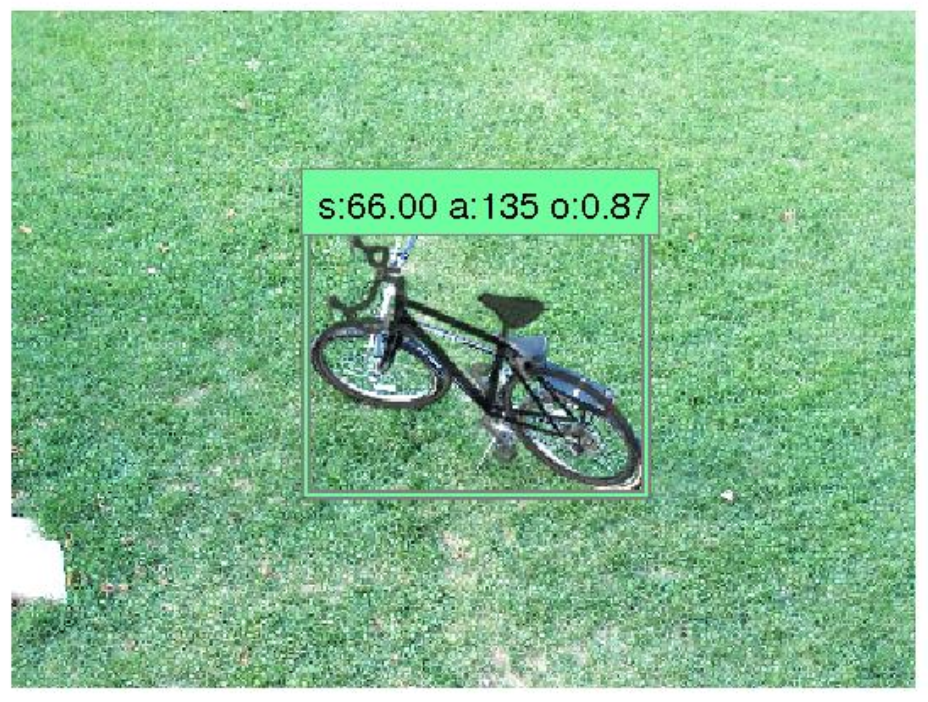
\includegraphics[width=0.35\linewidth]{car_3dobject/7.png} &   
  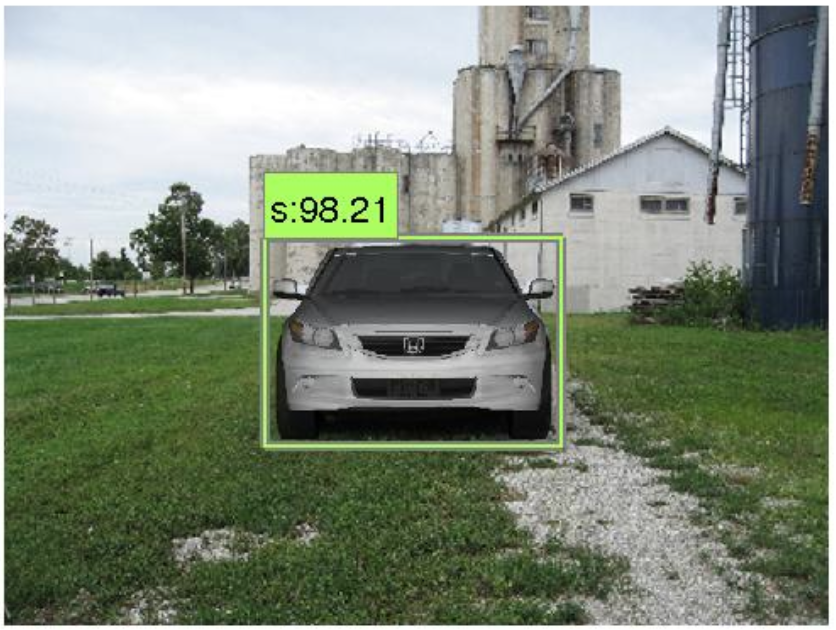
\includegraphics[width=0.35\linewidth]{car_3dobject/8.png}\\ [-15pt]
%   (a) & (b) \\[0pt]
  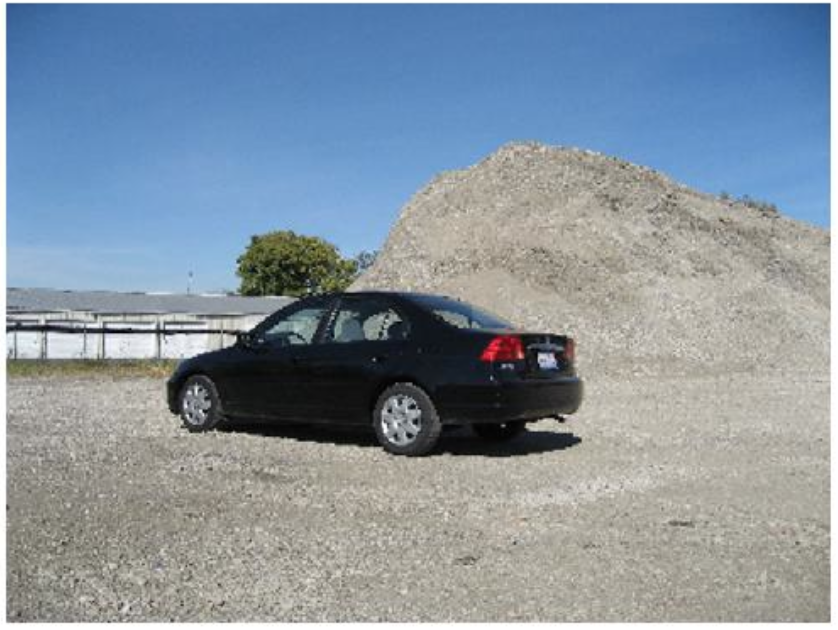
\includegraphics[width=0.35\linewidth]{car_3dobject/11.png} &   
  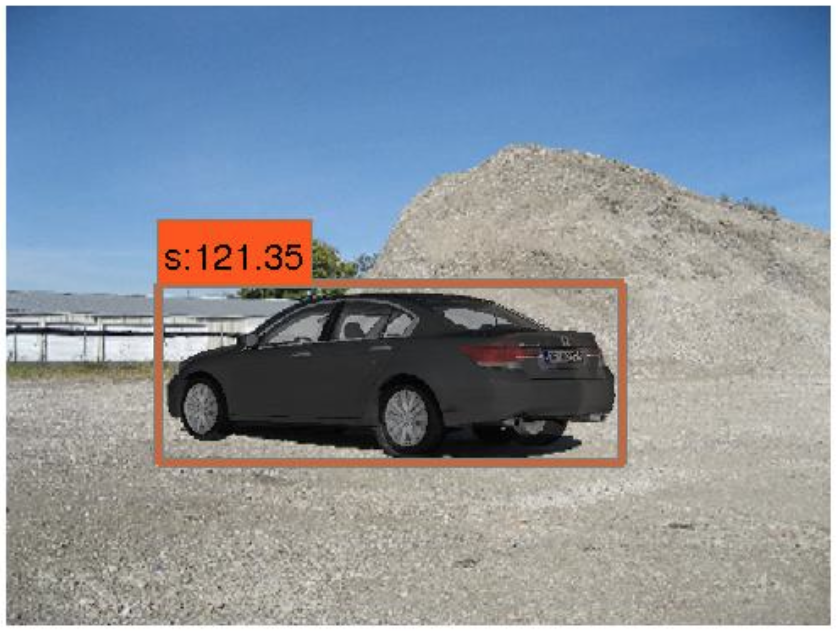
\includegraphics[width=0.35\linewidth]{car_3dobject/12.png}\\ [-5pt]
%  (c) & (d) \\[0pt]
\end{tabular}
\end{center}
\caption{Detection results on 3D Object
  Classes~\cite{Savarese07}. Original image (left) and detection
  result overlaid on top (right).}% with a bounding box and corresponding confidence score (right).}
  \label{fig:3dobject_vis}
\end{figure}


% Also, we evaluated our method on PASCAL 2007 dataset.
% 
% \begin{table}[!htbp]
%   \begin{center}
%   \begin{tabular}{|c|c|c|c|c|}
%     \hline
%      AP &    Ours &    ELDA \cite{Hariharan12} & ESVM \cite{Malisiewicz11} & VOCDPM \cite{Pepik12} \\
%     \hline\hline
%     car      & 27.          &  38.4  & 40.1    &65.7  \\ 
%     bicycle  & 43.74 & 41      &  40.7   & 61.3   \\
%     \hline
%     \end{tabular}
%   \end{center}
%   \caption{Average Precision(AP) on PASCAL 2007 dataset. Though we do not need any training images and made templates in few minues, it performs on par with state of the art detector yet it gives high quality 2D-3D matching.}
%   \label{tab:pascal07}
% \end{table}

\subsection{Enriching Existing Detections}
%\subsection{Fine-Tuning and Viewpoint Estimation}
\label{sec:exp_enrich}
In this section, we use our method to enrich the detections provided
by existing, high-performance object detectors with additional output
in the form a 3D pose, focal length, and 3D CAD model exemplar shape.
% High performance object detectors usually generalizes very well. It
% can handle various intraclass variability, viewpoint change and
% occlusion. However due to this high generalization, sometimes it is
% very difficult to get accurate pose, category or 2D-3D matching. Our
% method, specialized in giving such accurate information, can be
% applied on any generic object detectors to give high quality metadata.

To show such ability, we evaluate our method on the PASCAL3D+
dataset~\cite{Xiang14}. This dataset augments PASCAL 2012 images with
high quality viewpoint annotations thus is ideal to measure pose
estimation. The dataset proposes a new metric called Average Viewpoint
Precision (AVP) where it measures the area under viewpoint precision
and detection recall curve. The viewpoint is measured by azimuth
similarity. If the distance between predicted azimuth and ground truth
azimuth is below a certain threshold, the viewpoint is correct.
The baseline methods V-DPM~\cite{Xiang14} and
DPM-VOC+VP~\cite{Pepik12} reported on the PASCAL3D+ dataset are
variants of DPM~\cite{Felzenszwalb10} where each component of DPM
accounts for azimuth. Thus V-DPM and DPM-VOC+VP provide discrete
azimuths only whereas our method provides 3D viewpoint (yaw, pitch,
roll), CAD model instance (model index, rendering, depth) and focal length.
%
\begin{figure}[t]
 \begin{center}
    \setlength\tabcolsep{0pt}
    \begin{tabular}{ccc}
    % 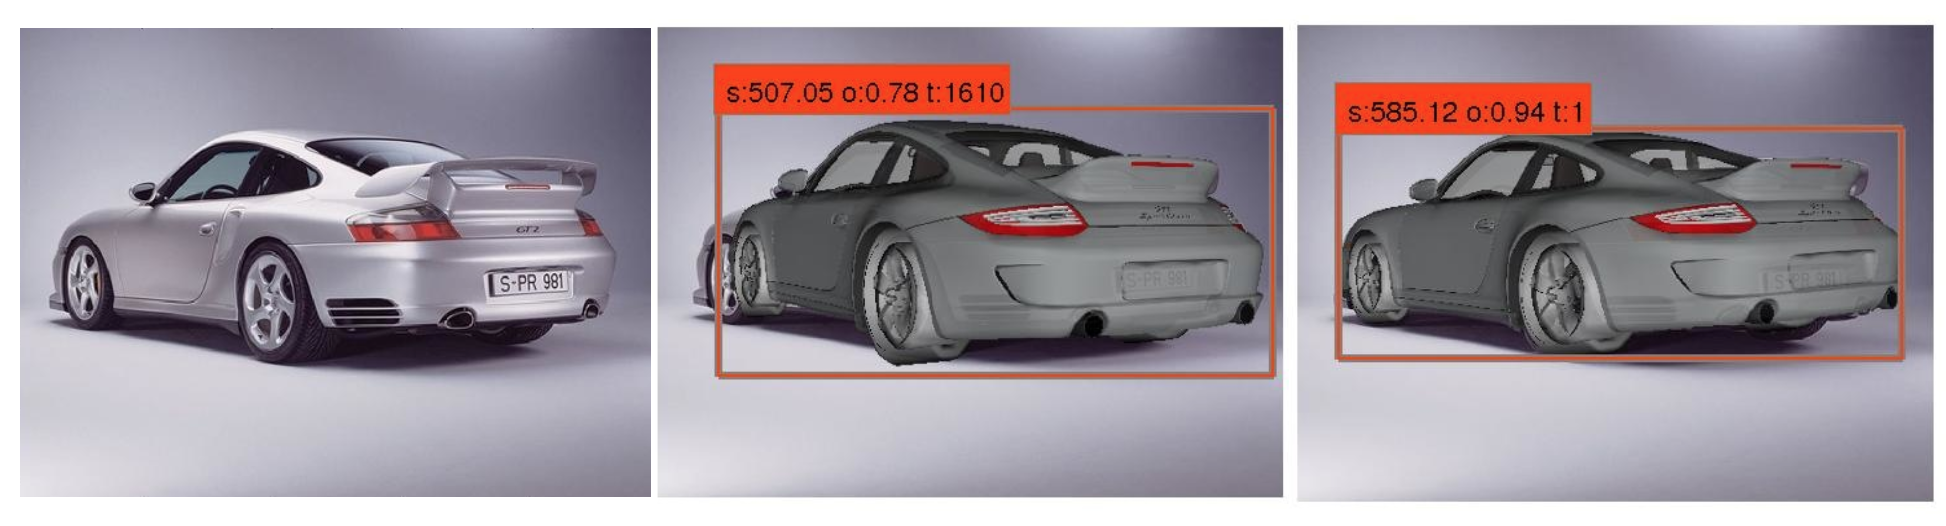
\includegraphics[width=0.9\linewidth]{tuning} 
   \includegraphics[width=0.33\linewidth]{tuning/1_sm.png} &
   \includegraphics[width=0.33\linewidth]{tuning/2_sm.png} &
   \includegraphics[width=0.33\linewidth]{tuning/3_sm.png} \\[-5pt]
%   (a) & (b) & (c)\\
   \includegraphics[width=0.33\linewidth]{tuning/4_sm.png} &
   \includegraphics[width=0.33\linewidth]{tuning/5_sm.png} &
   \includegraphics[width=0.33\linewidth]{tuning/6_sm.png} \\[-5pt]
%   (d) & (e) & (f)\\
   \end{tabular}
 \end{center}
 \caption{Effect of fine tuning. (left) original image, (middle) initial detection, (right) continuous fine tuning using Single-Component Metropolis Hastings}
 \label{fig:tuning}
\end{figure}

\vspace{-0.1in}
\paragraph{Setup.}
We use detection bounding boxes provided by both object detectors and
 use our method to perform fine-grained viewpoint estimation. We use
detection bounding boxes from two different methods:
DPM-VOC+VP~\cite{Pepik12} and R-CNN~\cite{Girshick14}, both in their
variants trained on 8 viewpoint categories, since these perform best
in terms of AP. For both cases,
we use the original score for plotting precision-recall curves
(meaning that we can not improve over their AP). We revert back to a default
viewpoint prediction ($0$ angles) in case the confidence of our
method falls below a threshold.

For both cases, we compare the performance of a discrete incarnation
of our method (Sect.~\ref{sec:approach}) and our full model, including the
fine-tuning based on MCMC (Sect.~\ref{sec:fine}).

Quantitative results are given in Tab.~\ref{tab:pascal12} in terms of
AP and AVP and in Fig.~\ref{fig:car_cnn_ap} in terms of
precision-recall plots and viewpoint confusion matrices. Example
outputs of our method applied to candidate object detections are given
in Fig.~\ref{fig:pascal12cnn}, and the effect of fine-tuning is
visualized in Fig.~\ref{fig:tuning}. More qualitative results can be found in the
supplemental material.


\vspace{-0.1in}
\paragraph{Results.}
%
In Tab.~\ref{tab:pascal12}, we make two main observations. First, we
see that adding our method to DPM-VOC+VP consistently improves
performance in terms of AVP, for both car and bicycle, and across all
viewpoint bins. This is already the case for our discrete method: the
improvement ranges from $0.3$ for bicycle-8v to $5.8$ for car-4v. 
%
Using the R-CNN as the base detector increases AVP even more, in
particular for the bicycle class: for bicycle-4v, our discrete method
improves over the corresponding DPM-VOC+VP result by $12.6$.

The second observation is that the fine-tuning based on MCMC can
indeed improve pose estimation performance slightly, e.g., by $1.1$
for bicycle-16v and using the DPM-VOC+VP as the base detector, or by
$1.1$ for bicycle-16v when using the R-CNN as the base detector.
%
In Fig.~\ref{fig:tuning}, we visualize the effect of fine-tuning
qualitatively for two different test images. In both cases, the
fine-tuned pose is a better visual match to the true 3D pose.
% We got significant improvement on viewpoint estimation by using our
% method on top of general purpose detectors. Note that our method
% estimates azimuth, elevation, in-plane rotation, focal length
% estimation, fine-grained categorization whereas V-DPM, VOC-DPM only
% estimate discrete viewpoints.

\begin{figure*}[t]
\setlength\tabcolsep{1pt}
\centering
\begin{tabular}{|ccccc|}
   \hline
  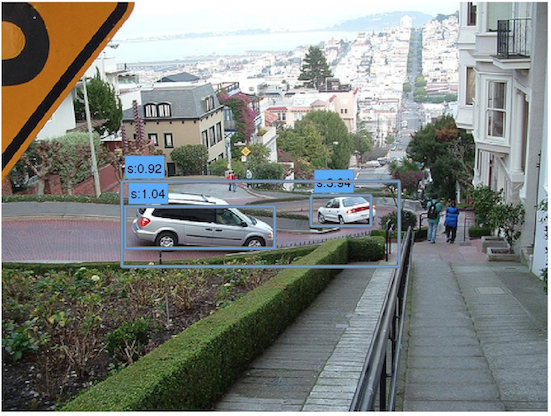
\includegraphics[width=0.24\textwidth]{car_cnn/1a.png} &   
  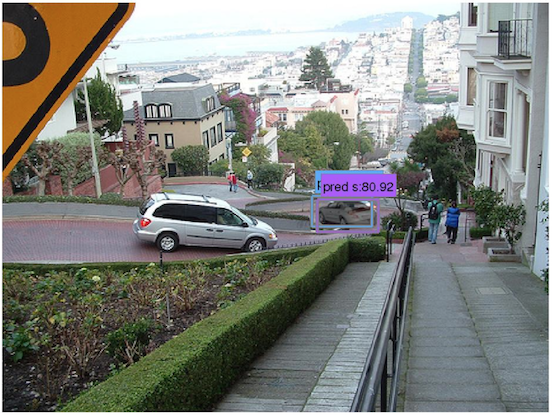
\includegraphics[width=0.24\textwidth]{car_cnn/1b.png} &   
  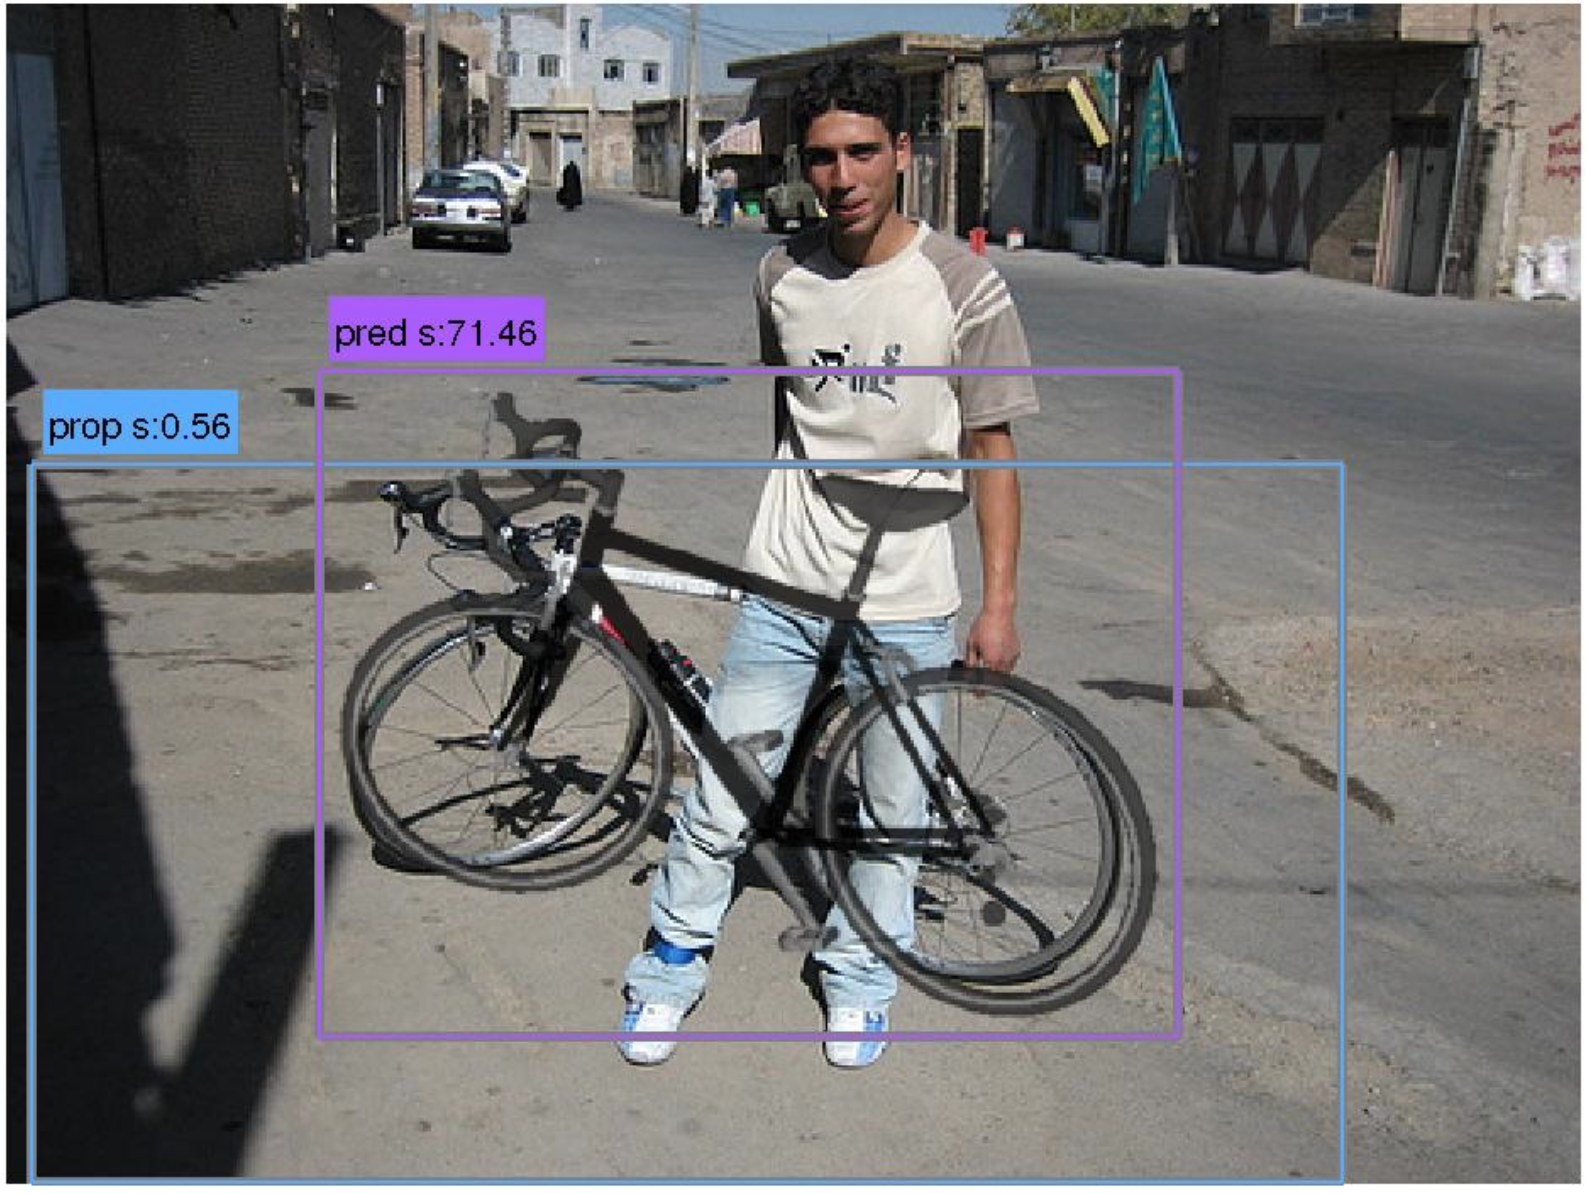
\includegraphics[width=0.24\textwidth]{car_cnn/1c.png} &   
  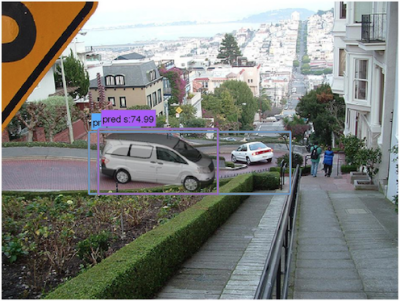
\includegraphics[width=0.24\textwidth]{car_cnn/1d.png}  \\  
   \hline
  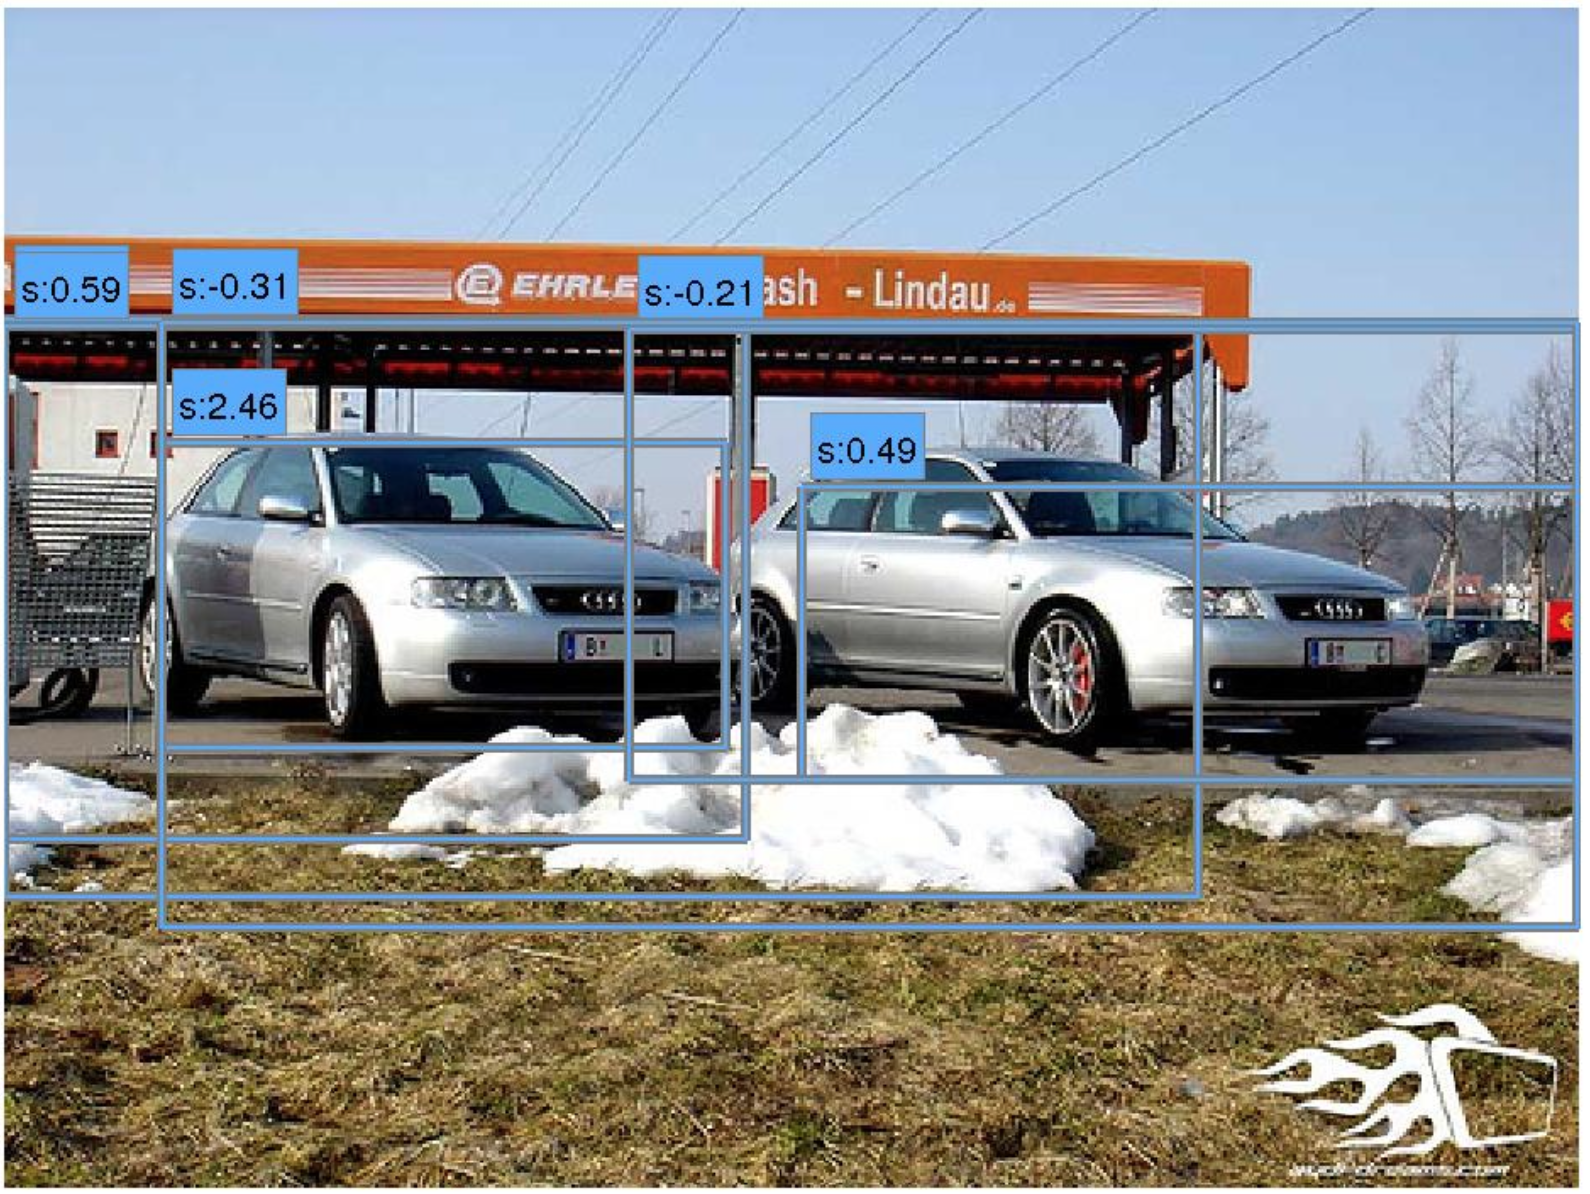
\includegraphics[width=0.24\textwidth]{car_cnn/2a.png} &   
  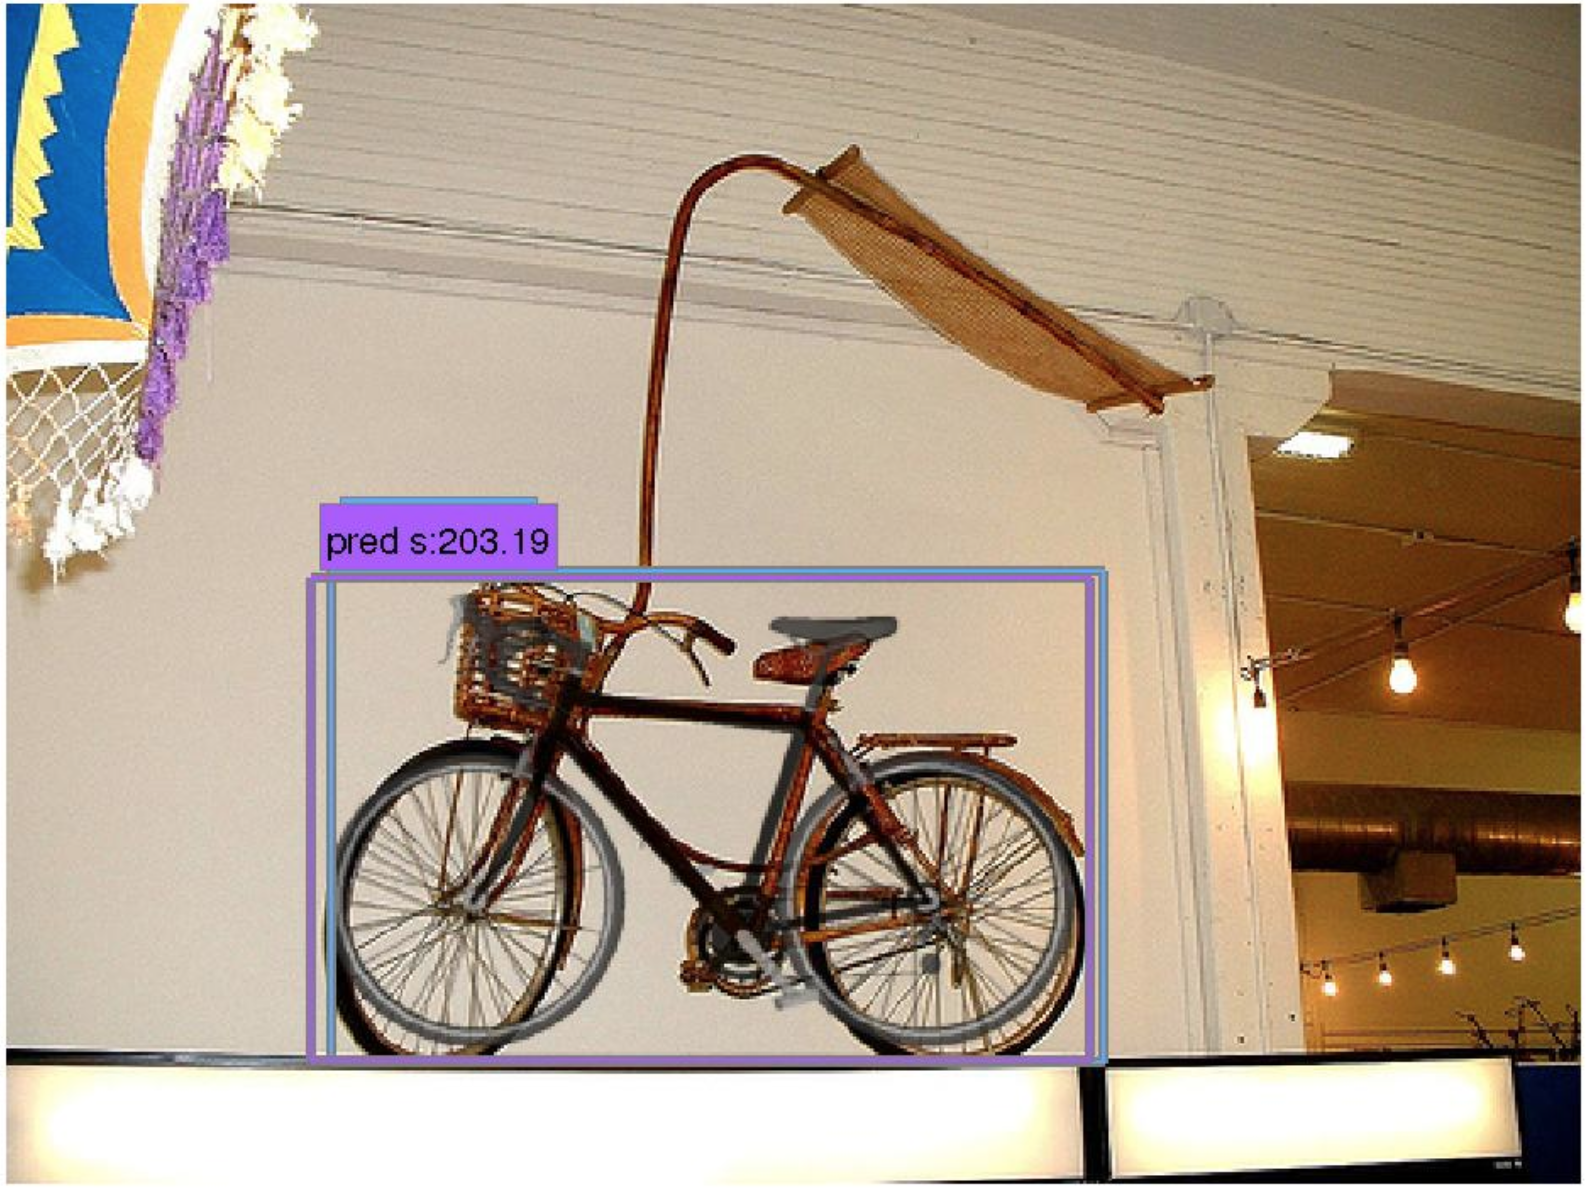
\includegraphics[width=0.24\textwidth]{car_cnn/2b.png} &   
  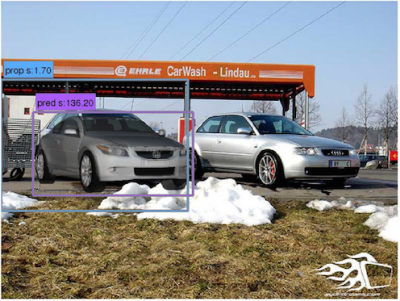
\includegraphics[width=0.24\textwidth]{car_cnn/2c.png} &   
  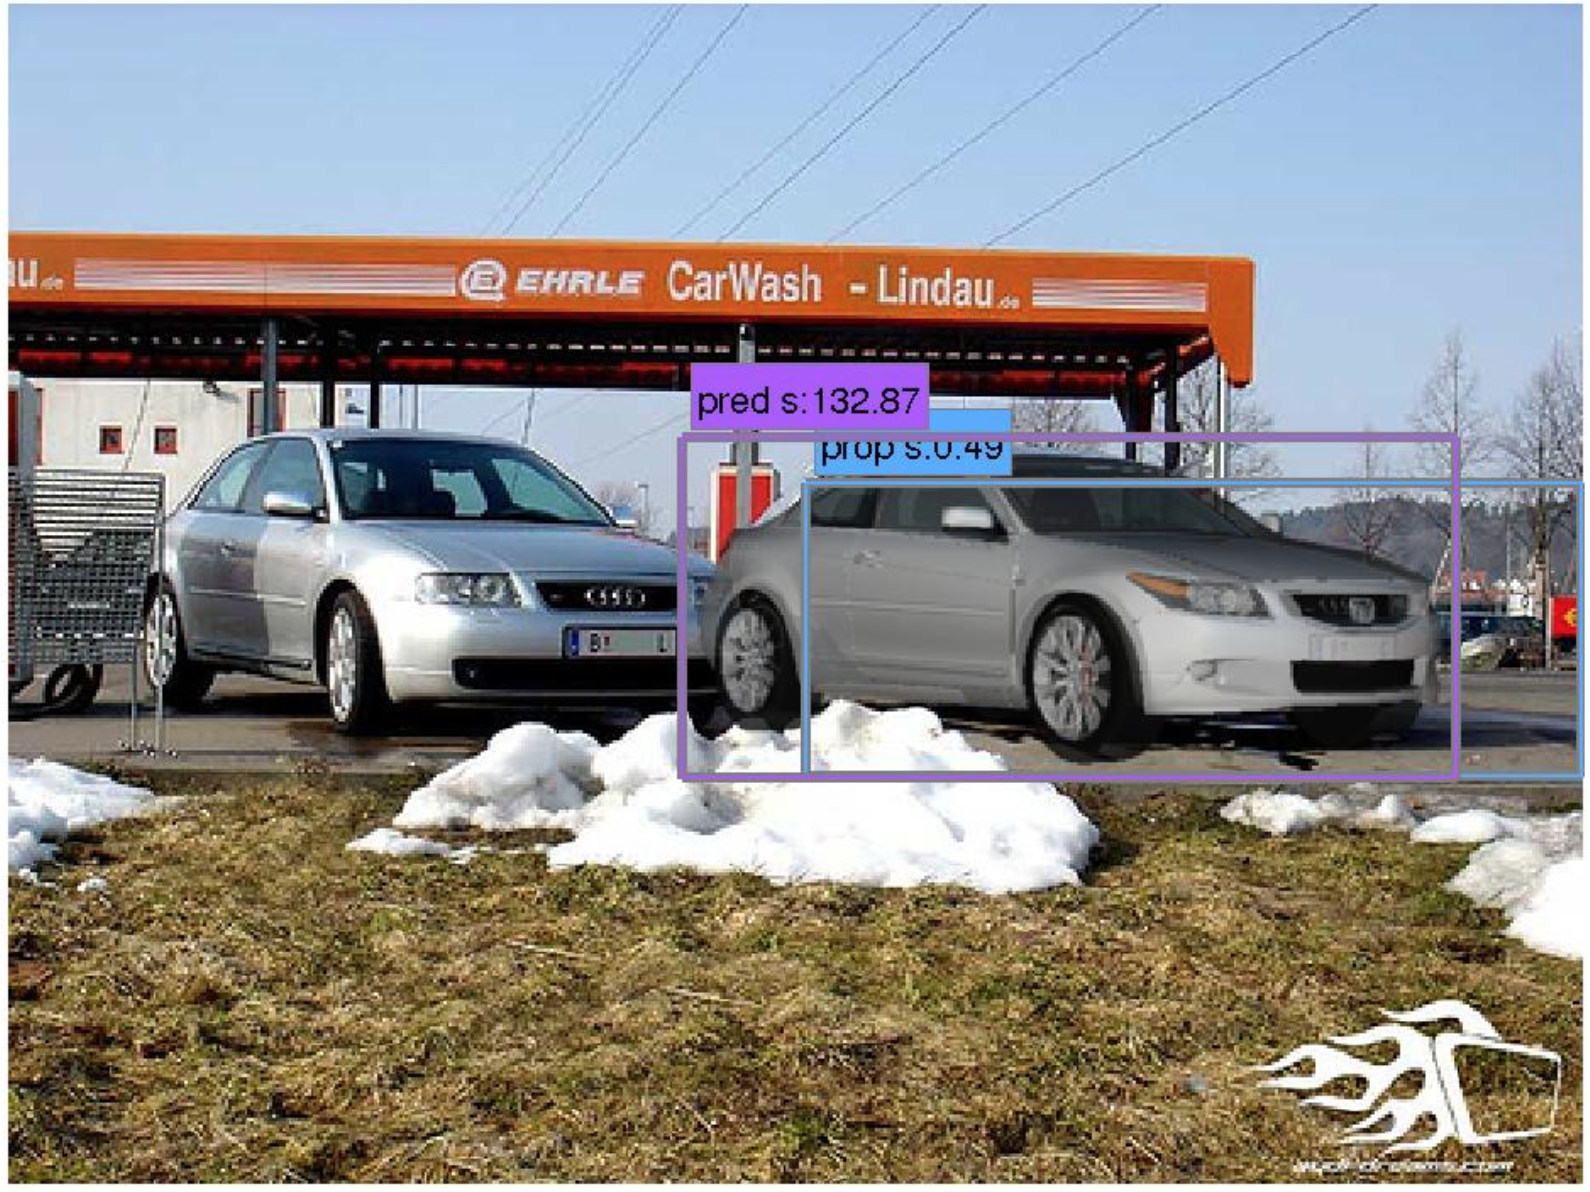
\includegraphics[width=0.24\textwidth]{car_cnn/2e.png}  \\  
   \hline
  \includegraphics[width=0.24\textwidth]{car_cnn/4a.png} &   
  \includegraphics[width=0.24\textwidth]{car_cnn/4b.png} &   
  \includegraphics[width=0.24\textwidth]{car_cnn/4c.png} &   
  \includegraphics[width=0.24\textwidth]{car_cnn/4d.png}  \\  
%    \hline
%   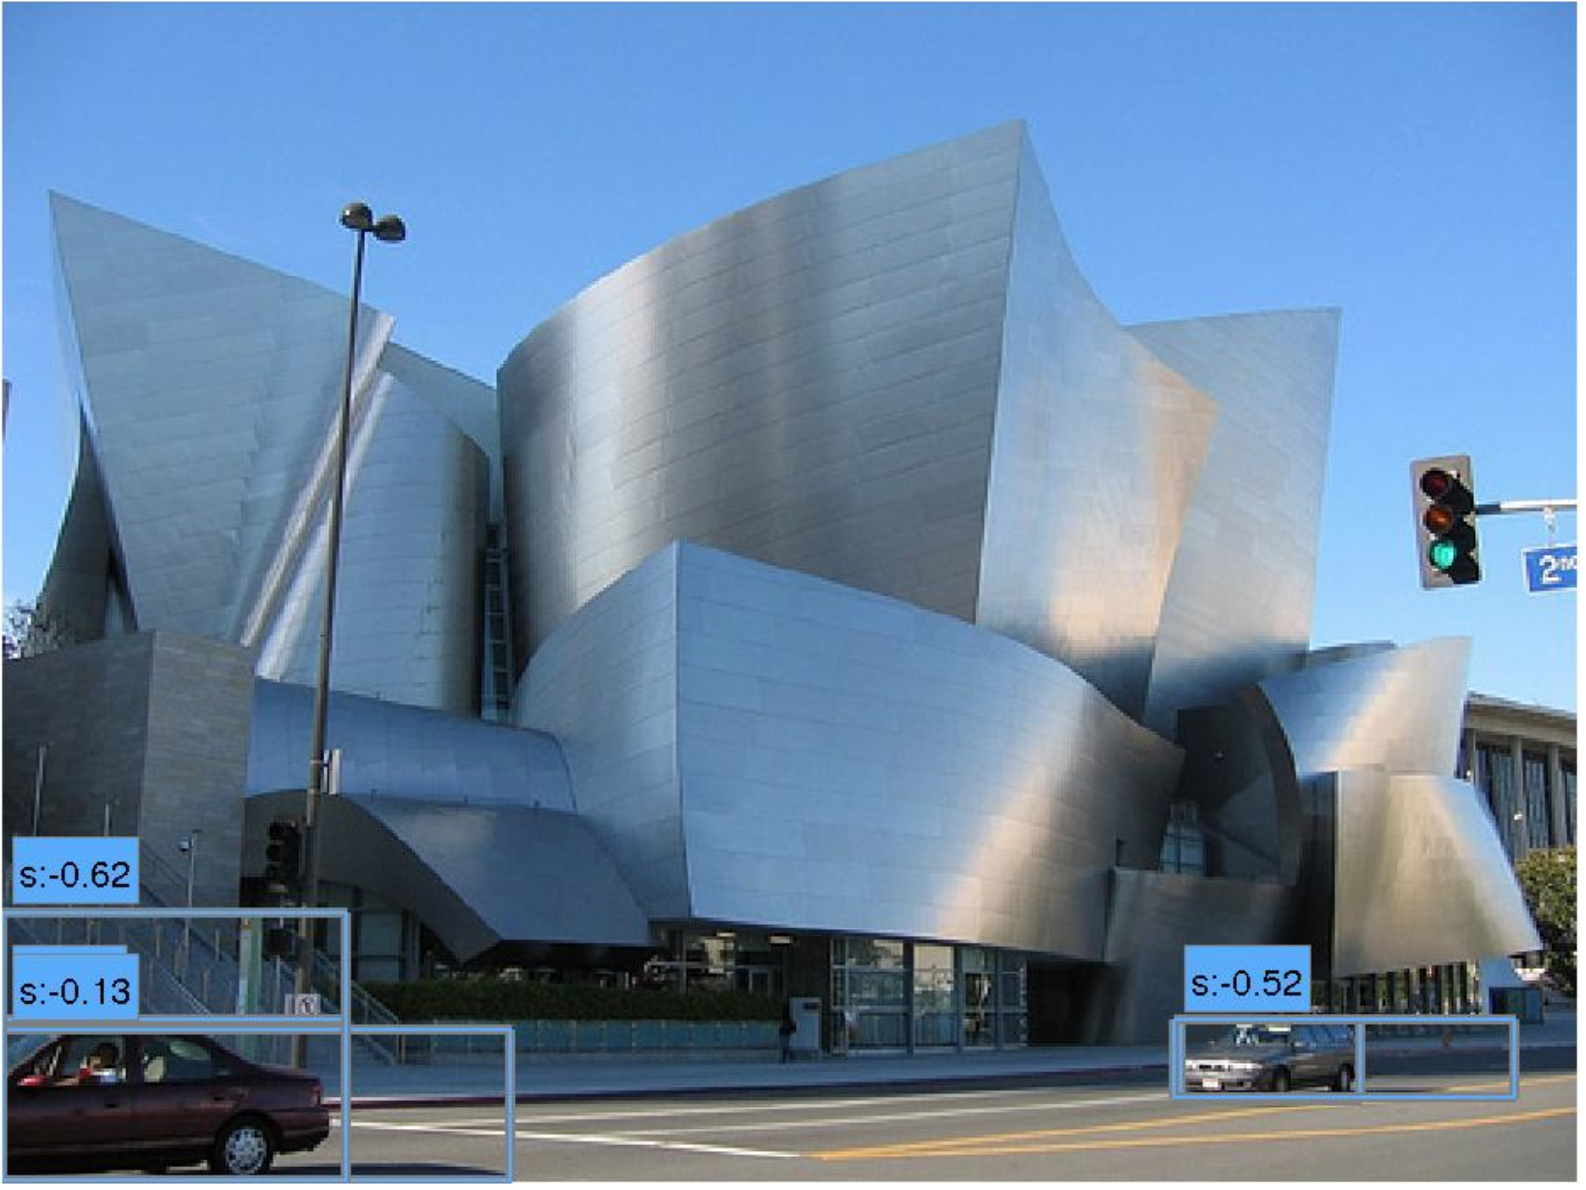
\includegraphics[width=0.24\textwidth]{car_cnn/10a.png} &   
%   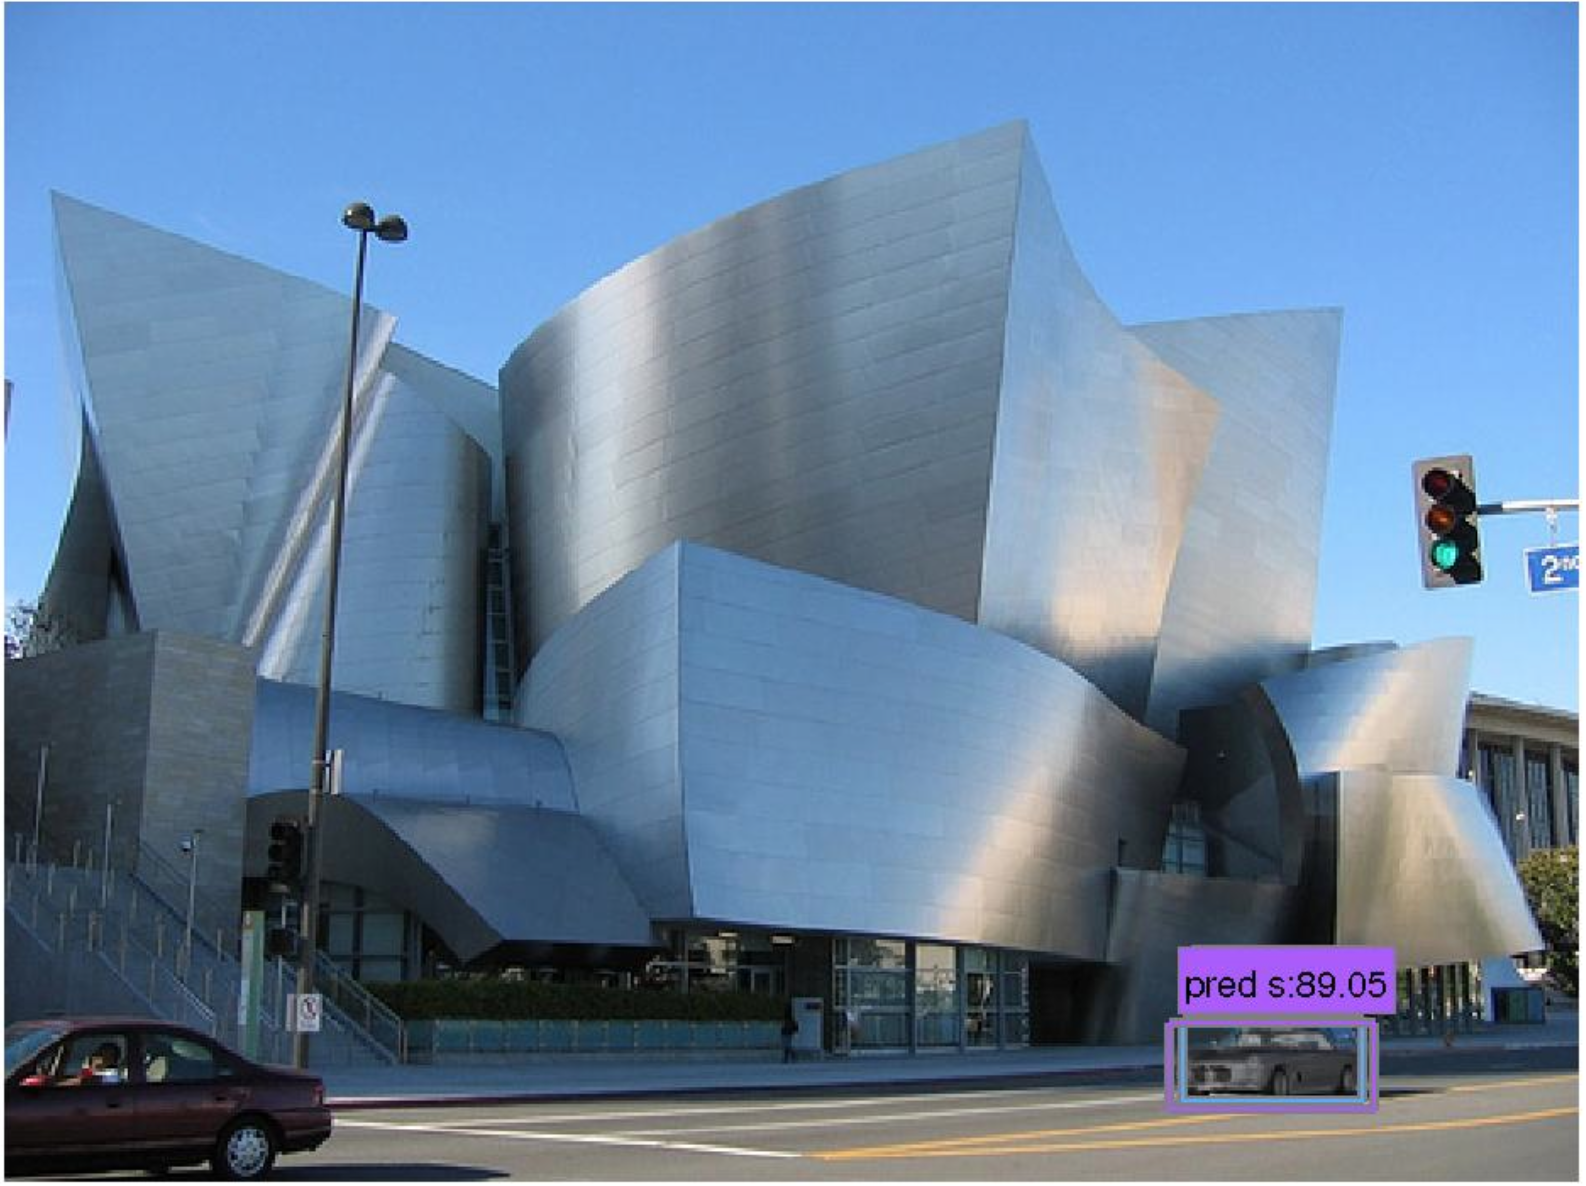
\includegraphics[width=0.24\textwidth]{car_cnn/10b.png} &   
%   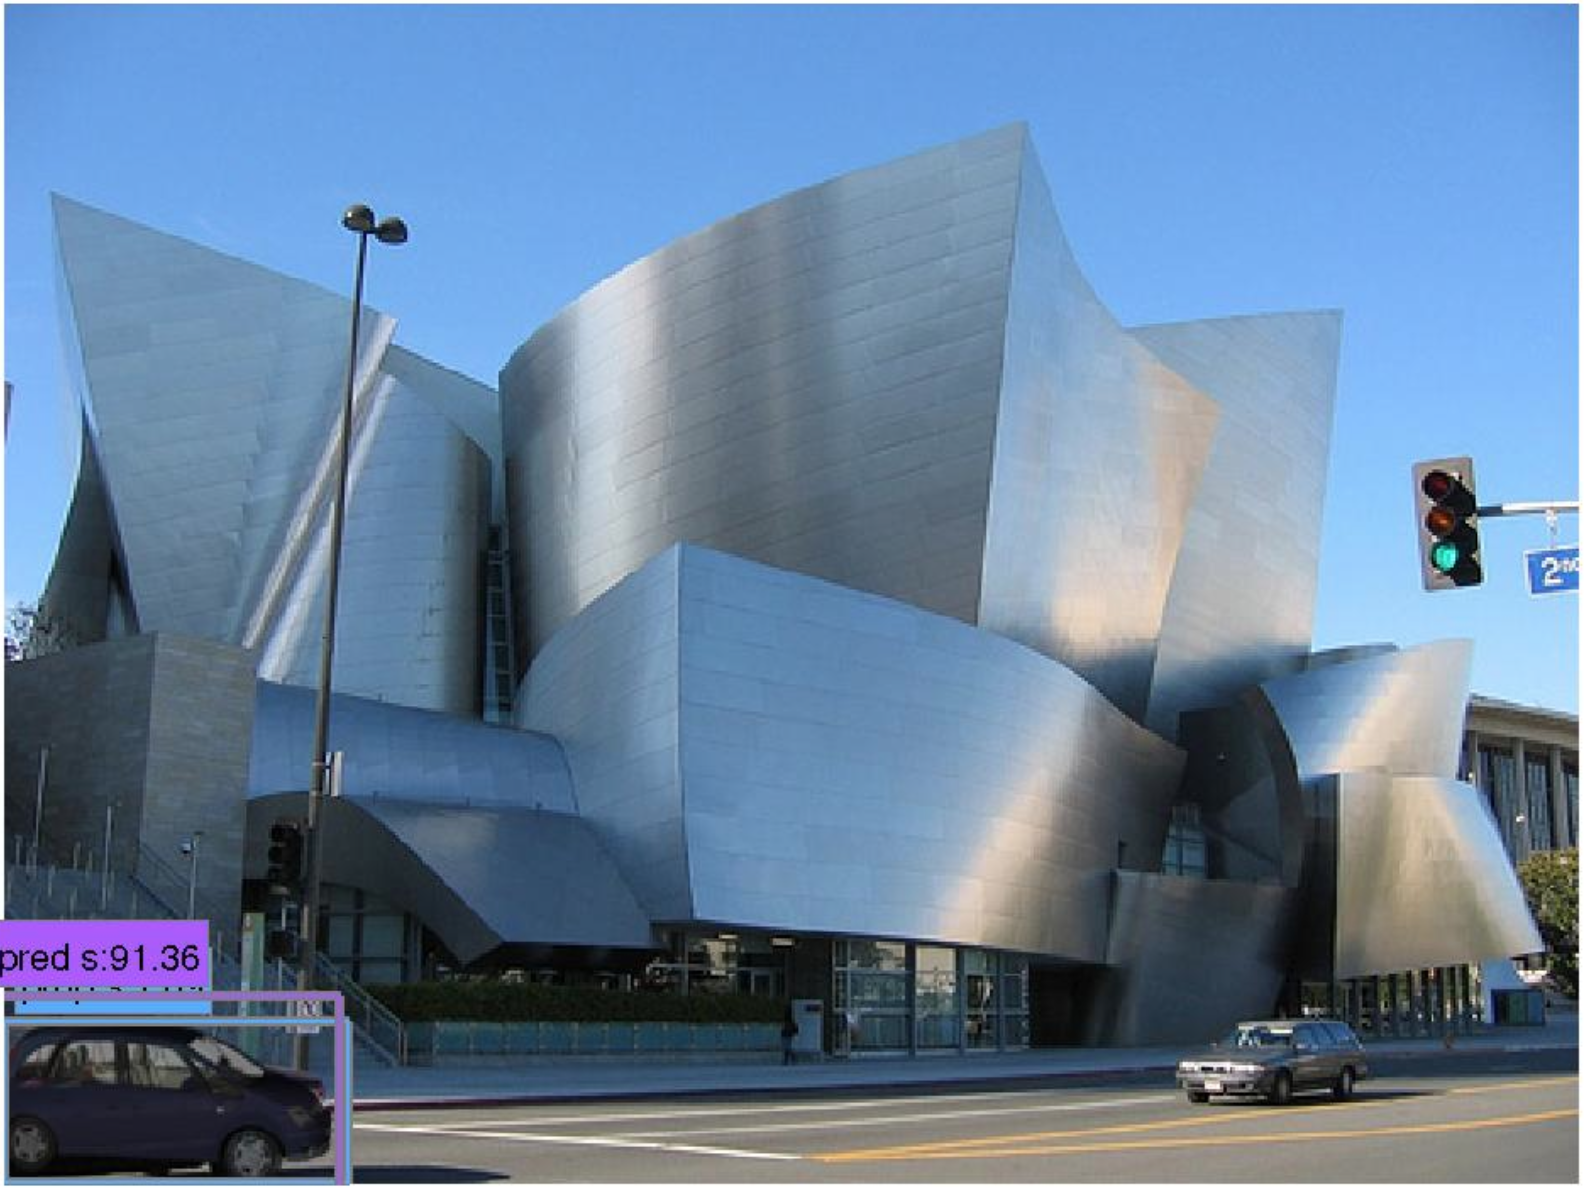
\includegraphics[width=0.24\textwidth]{car_cnn/10c.png} &   
%   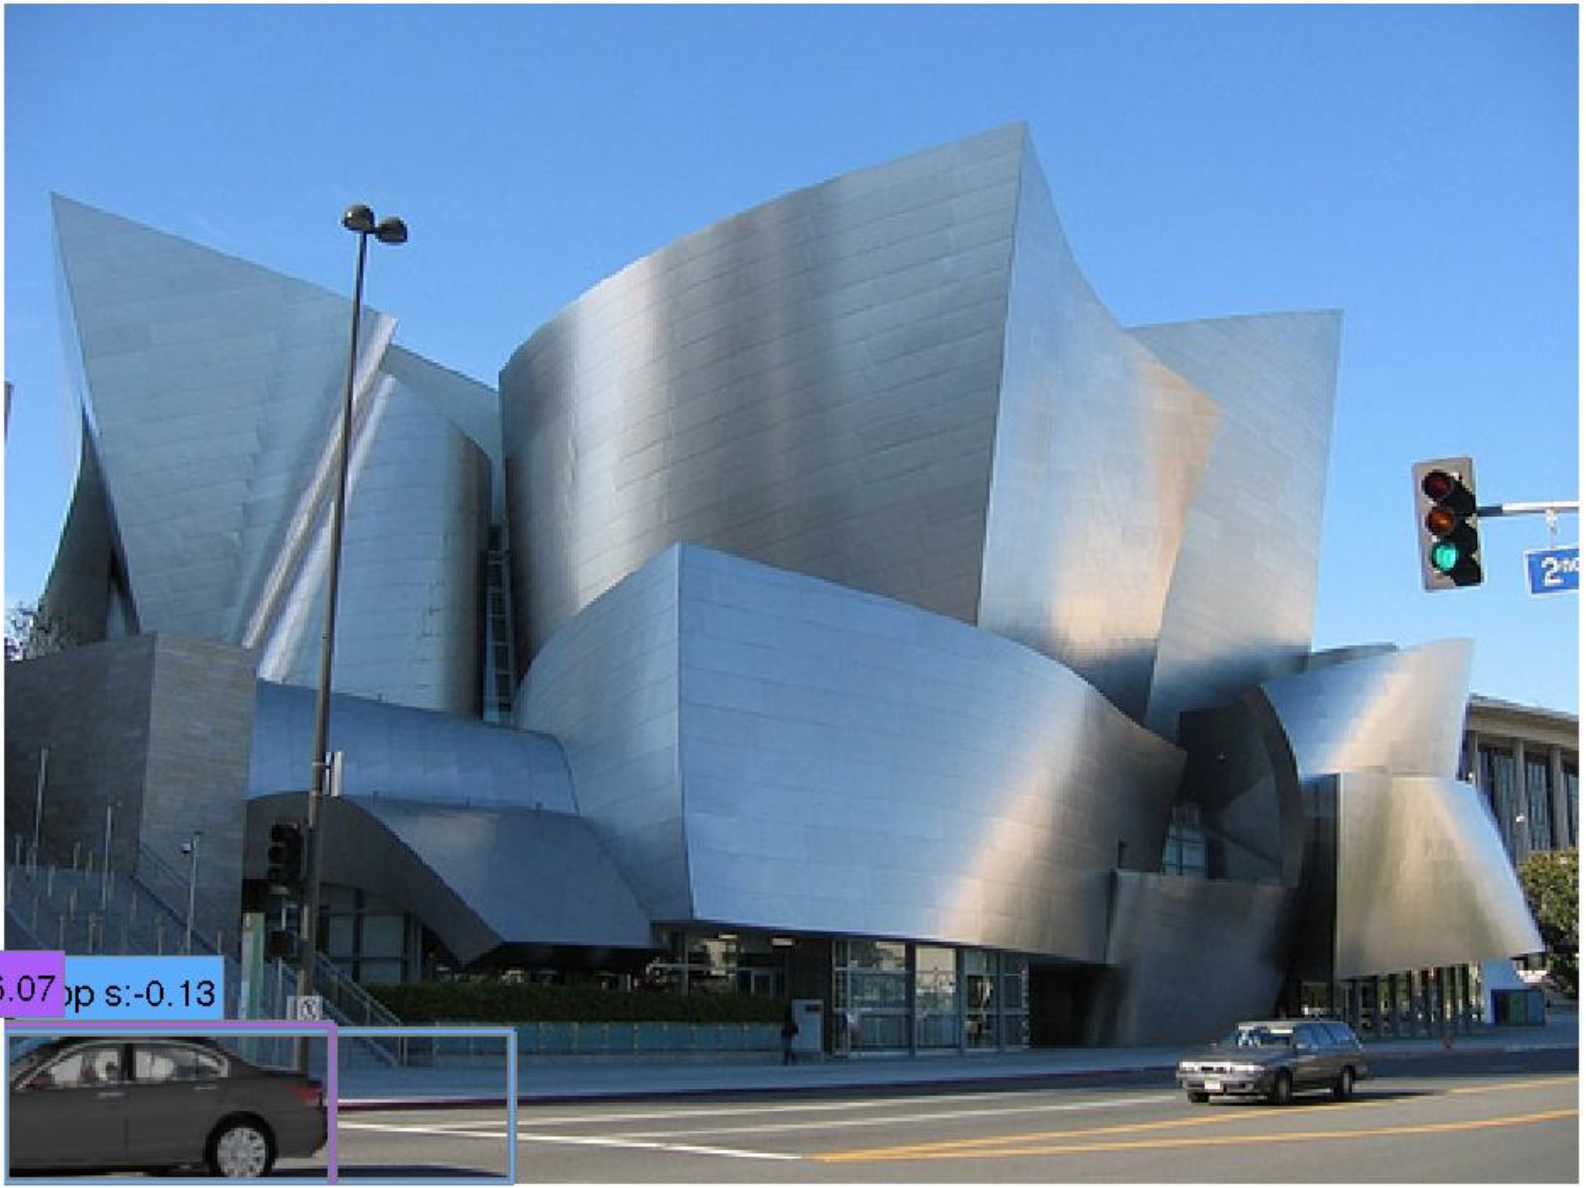
\includegraphics[width=0.24\textwidth]{car_cnn/10d.png}  \\  
%   \hline 
%   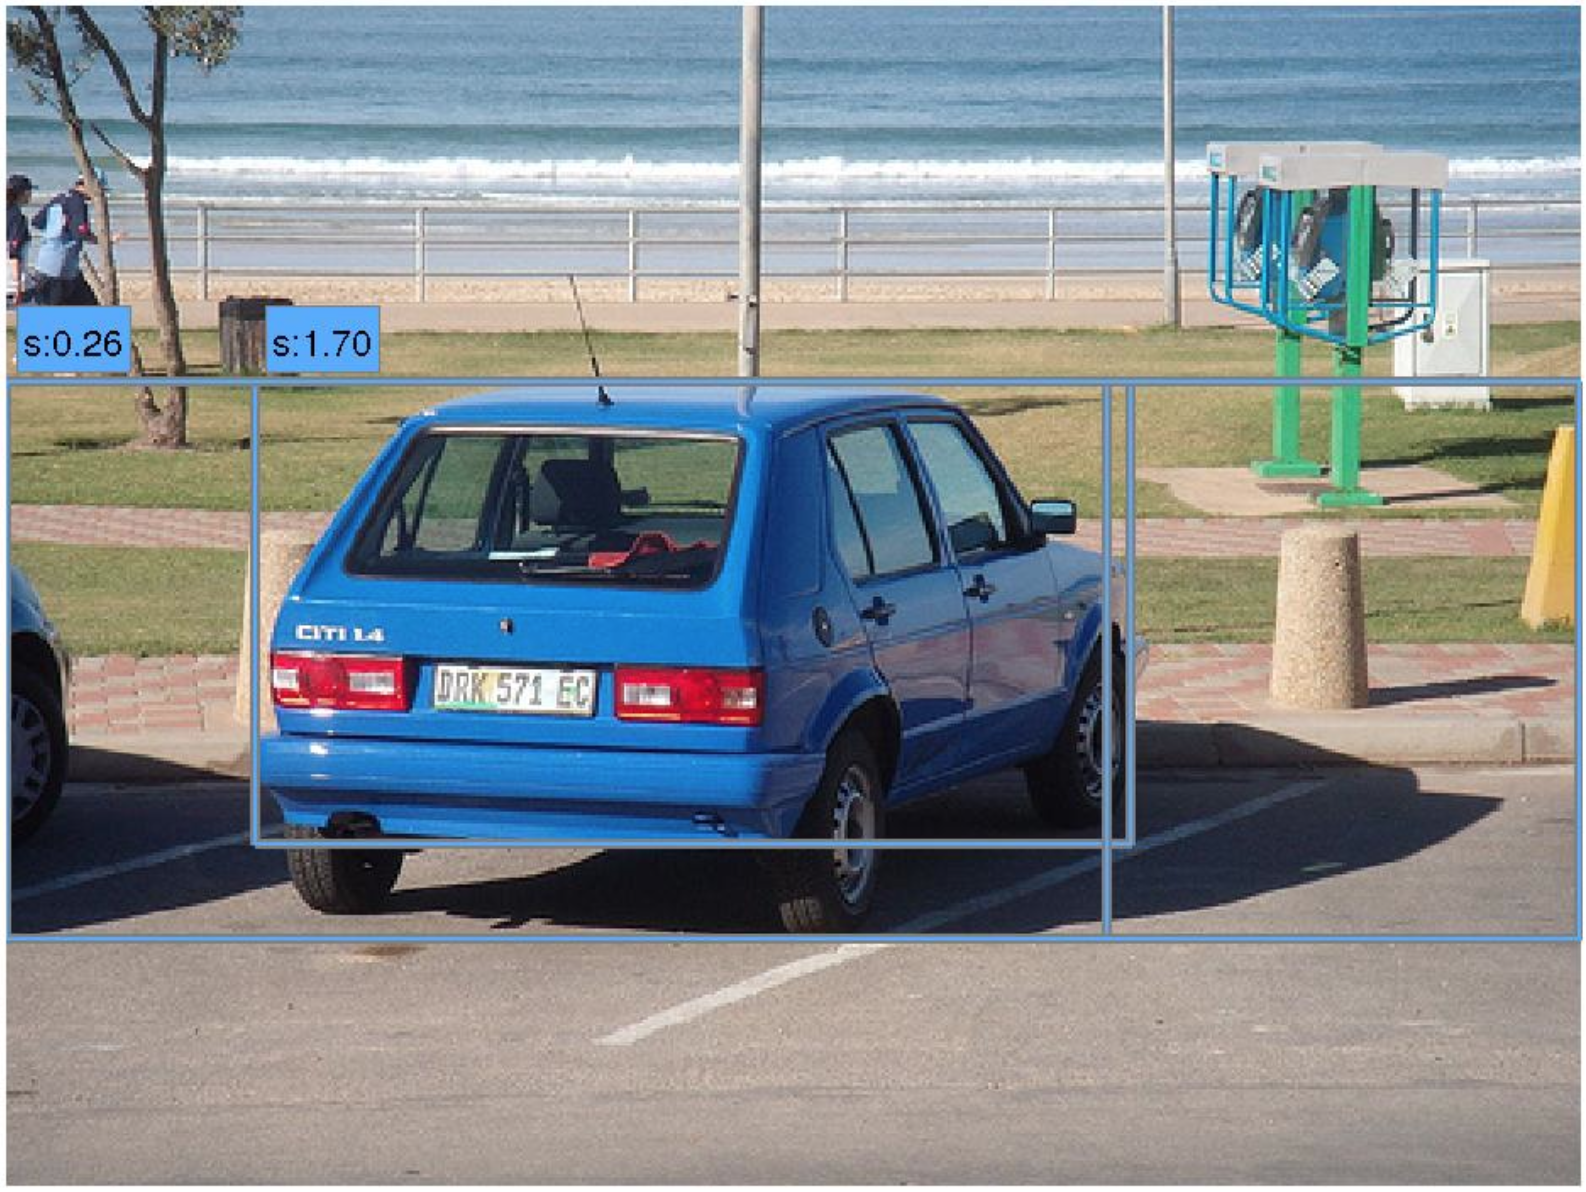
\includegraphics[width=0.24\textwidth]{bicycle_cnn/3a.png} &   
%   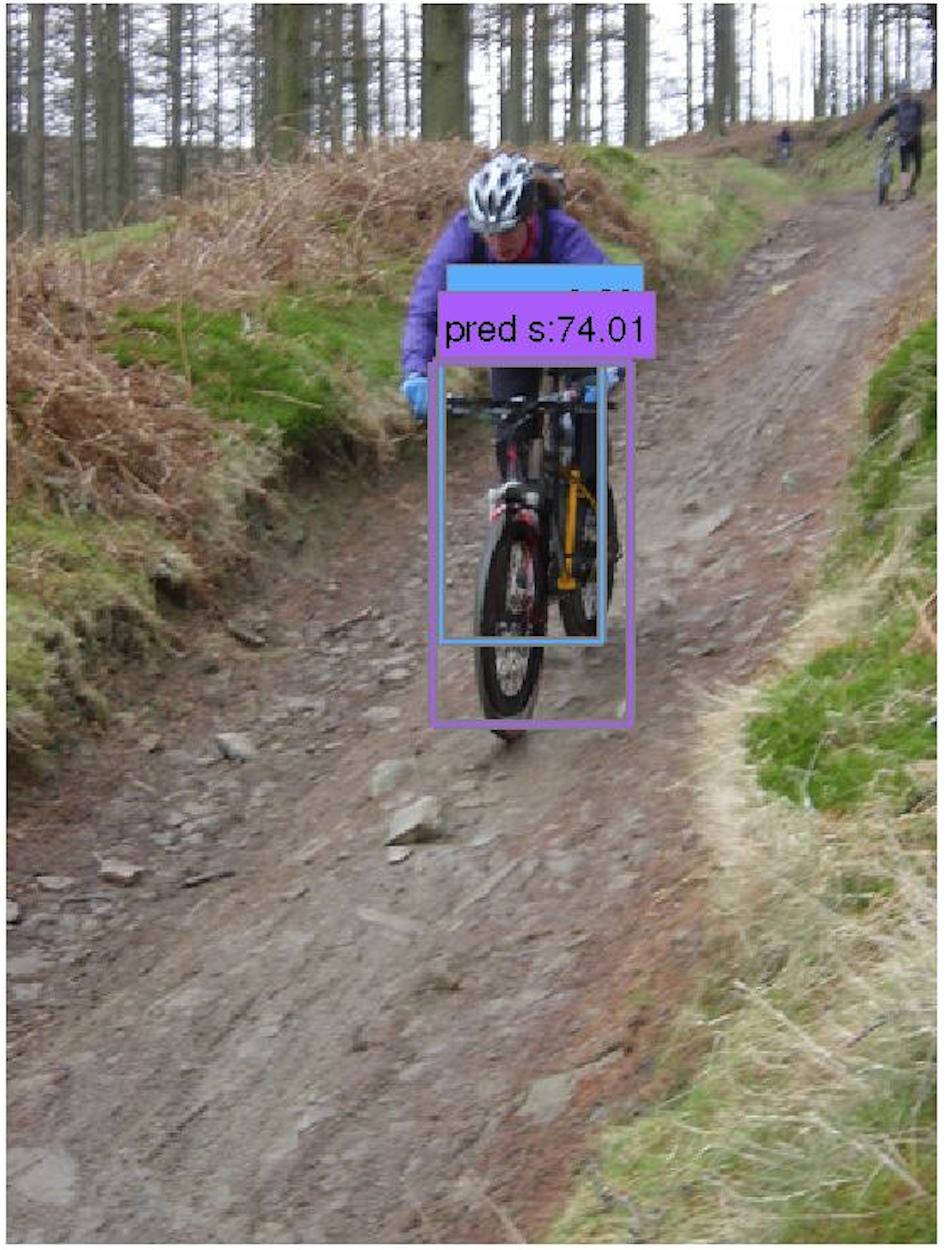
\includegraphics[width=0.24\textwidth]{bicycle_cnn/3b.png} &   
%   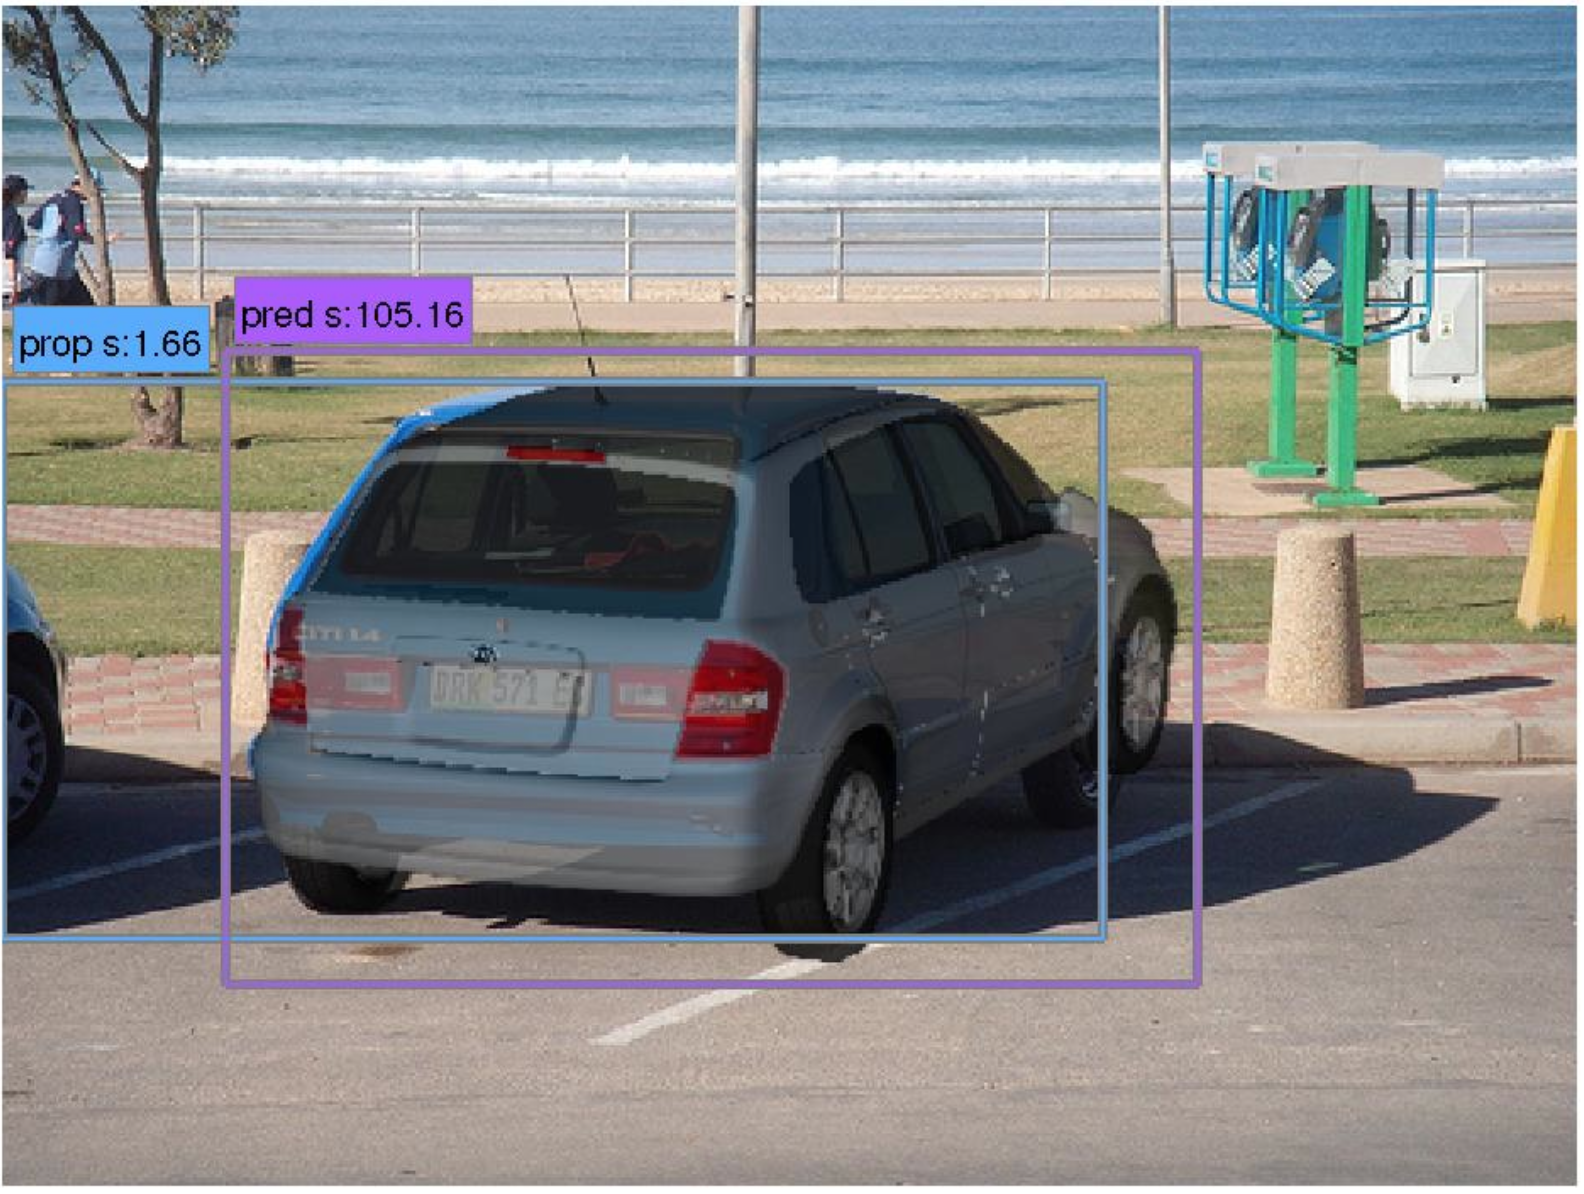
\includegraphics[width=0.24\textwidth]{bicycle_cnn/3c.png} &   
%   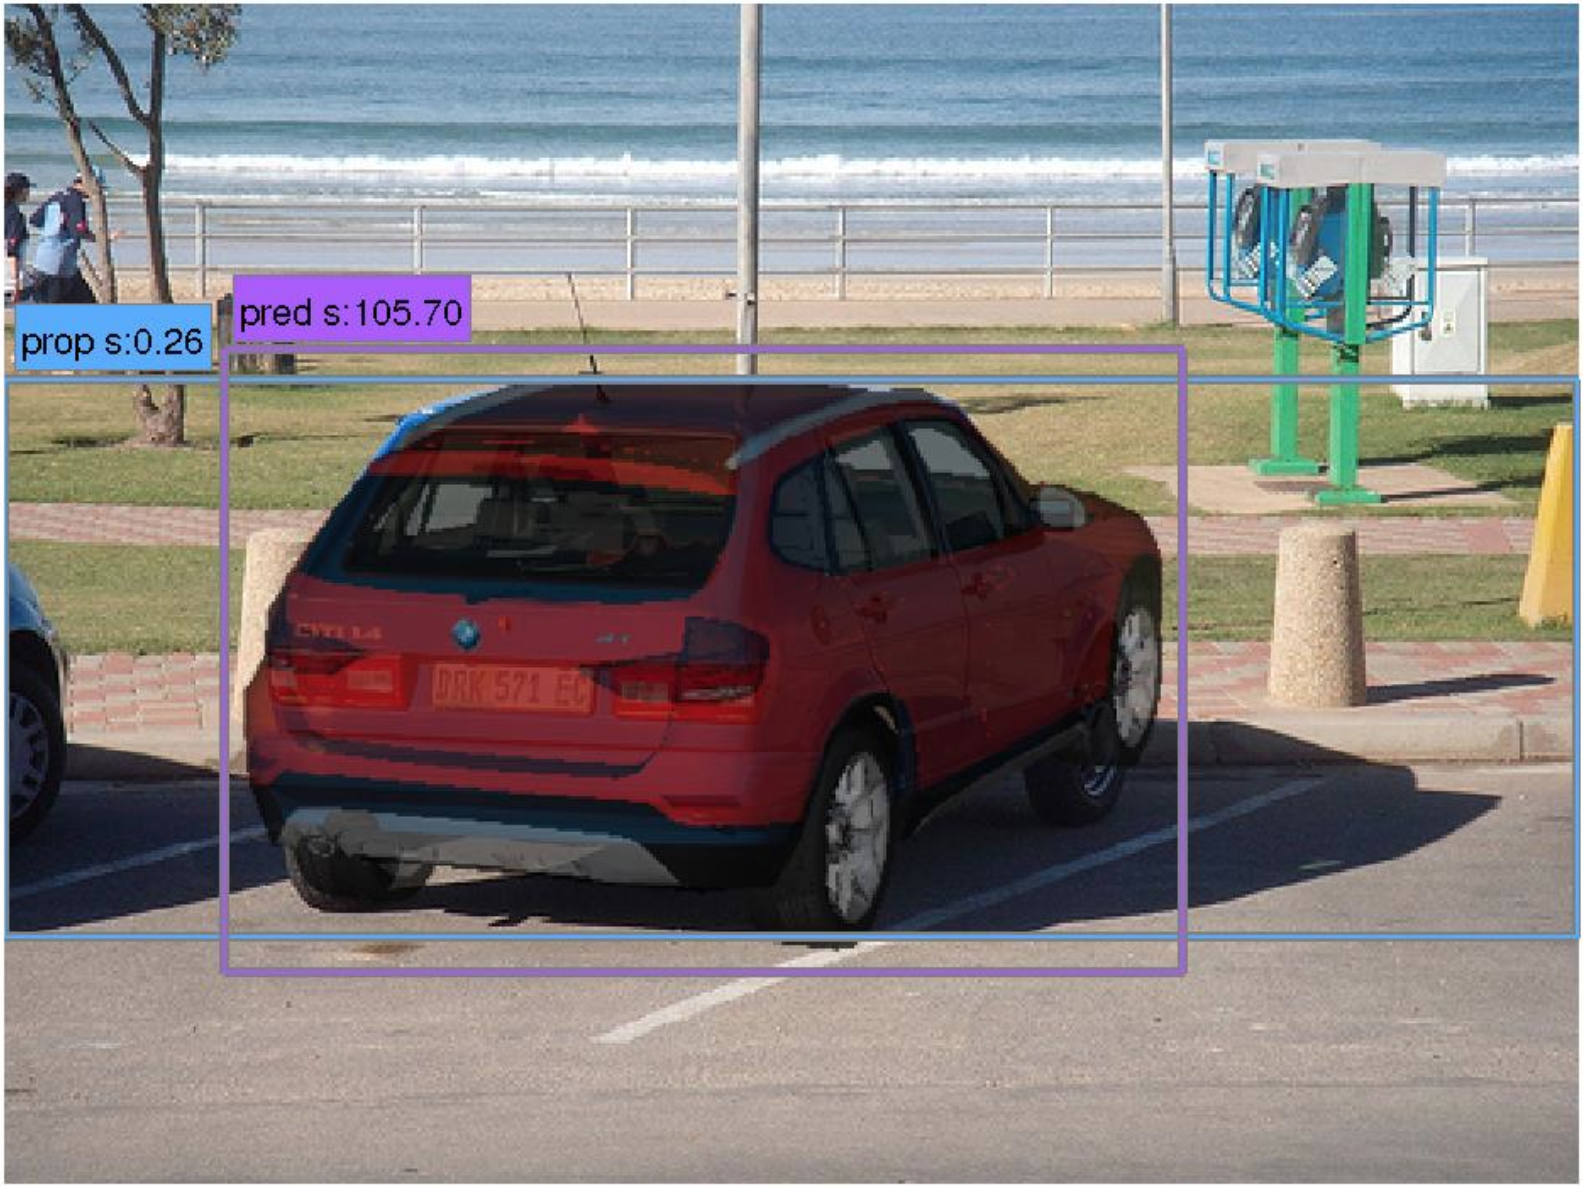
\includegraphics[width=0.24\textwidth]{bicycle_cnn/3d.png}  \\
%
% sorry no space
%  \hline
%  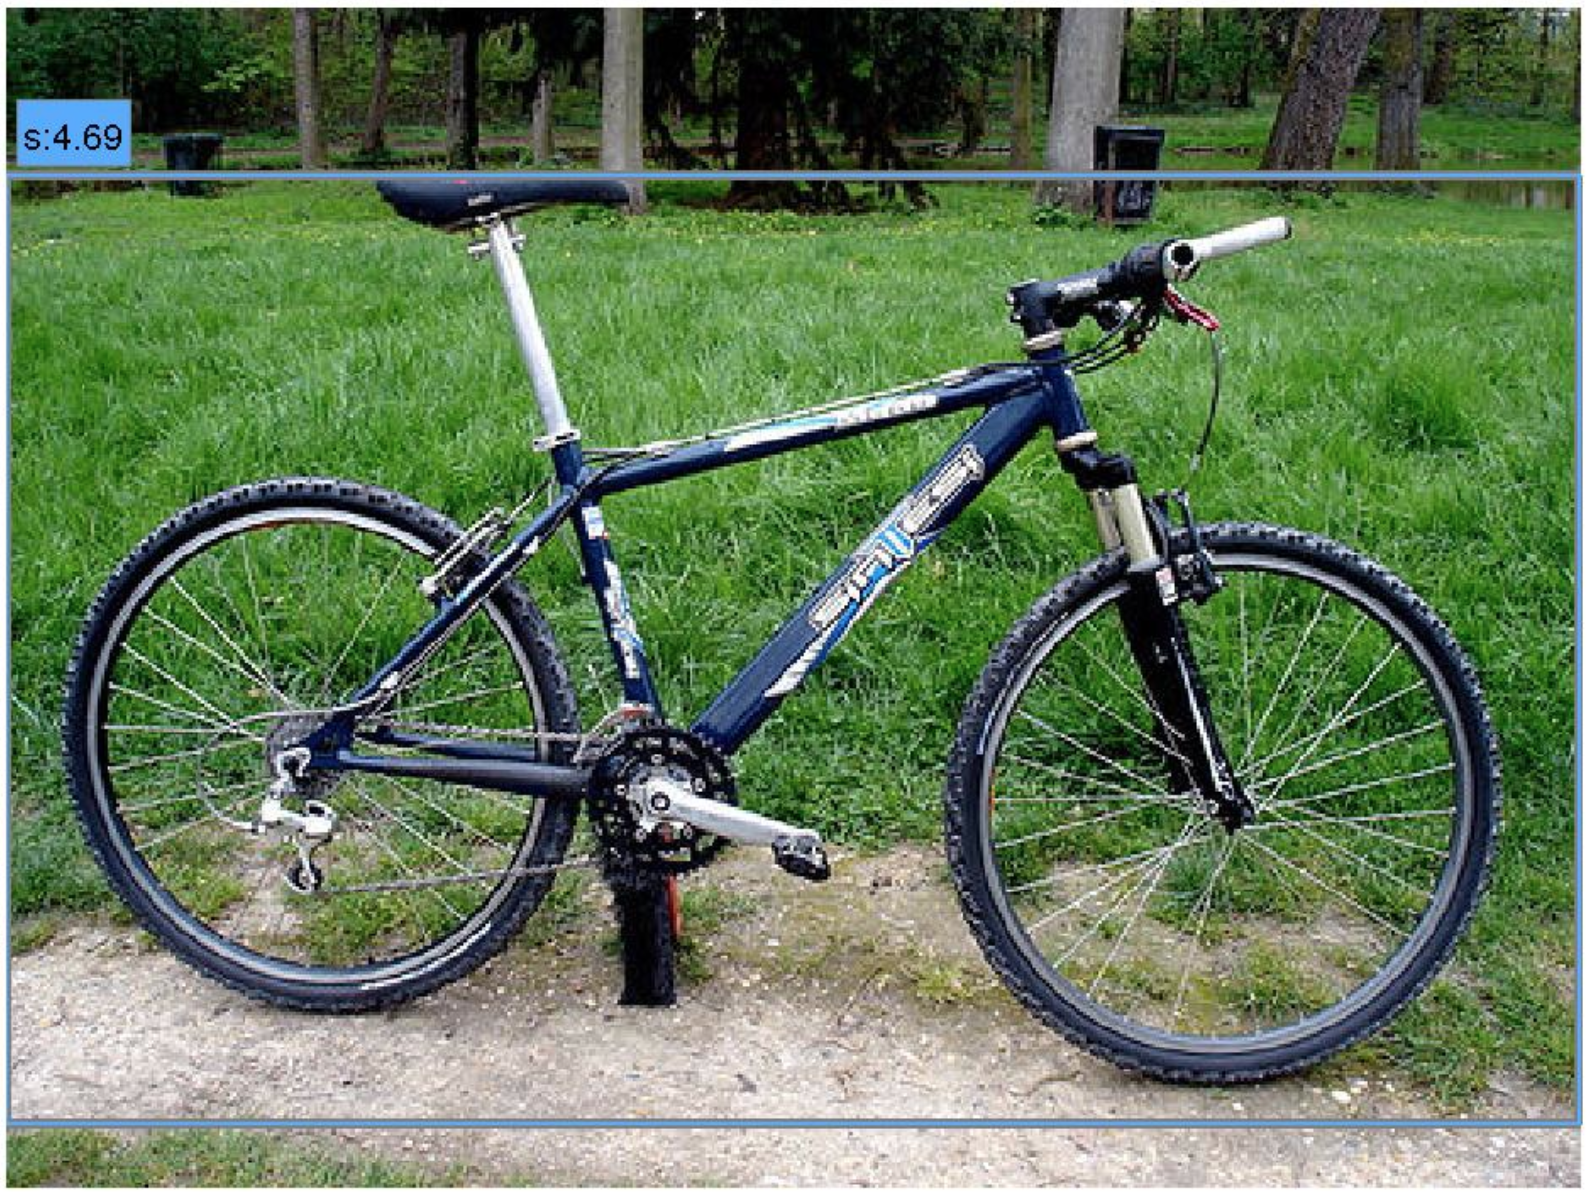
\includegraphics[width=0.24\textwidth]{bicycle_cnn/7a.png} &   
%  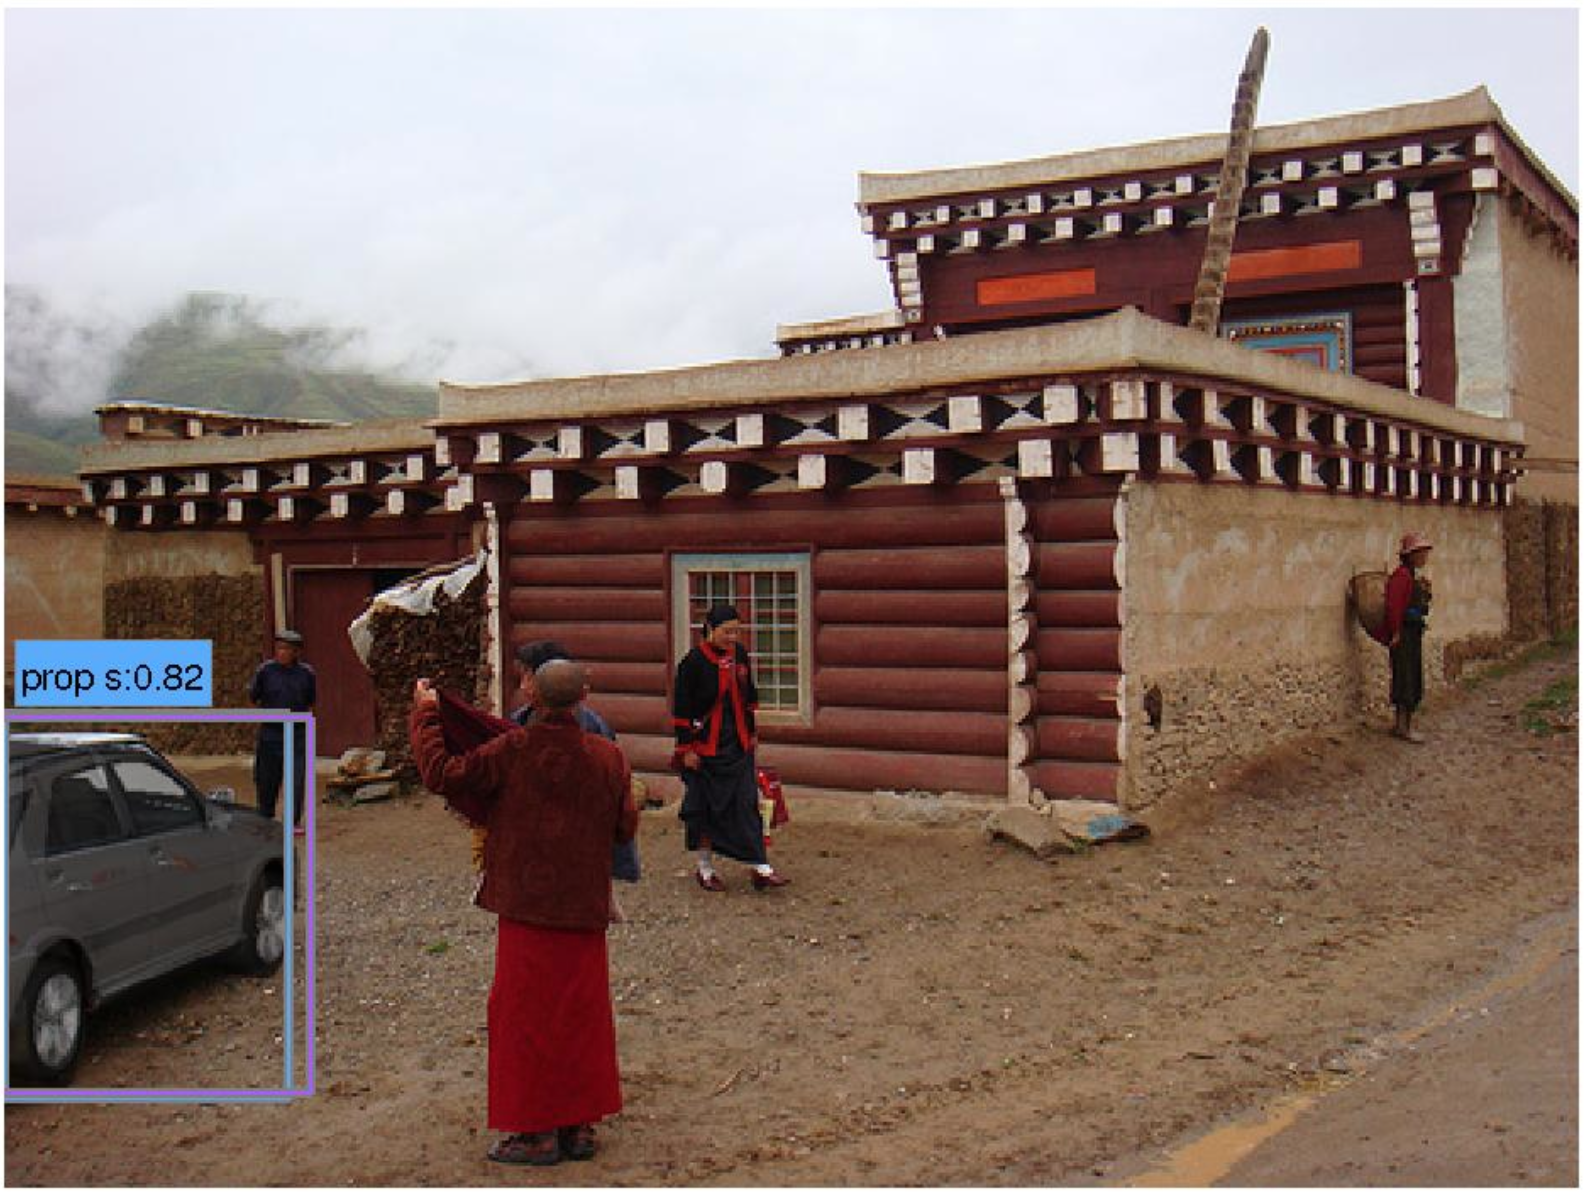
\includegraphics[width=0.24\textwidth]{bicycle_cnn/7b.png} &   
%  &\\
%  \hline
  \includegraphics[width=0.24\textwidth]{bicycle_cnn/4a.png} &   
  \includegraphics[width=0.24\textwidth]{bicycle_cnn/4b.png} &   
  \includegraphics[width=0.24\textwidth]{bicycle_cnn/4c.png} &   
  \includegraphics[width=0.24\textwidth]{bicycle_cnn/4d.png}  \\
  \hline
  CNN Proposals & \multicolumn{3}{|c|}{Our matching results on proposal bounding boxes} \\
  \hline
\end{tabular}
\caption{Example enriched bounding boxes. Given R-CNN~\cite{Girshick14}
  detection bounding boxes, our method predicted 2D-3D matching
  reasonably. The first column shows bounding boxes produced by R-CNN detection. Subsequent columns show the output of our method given this bounding box input. Blue boxes are R-CNN output and purple boxes are
  the tightest bounding box enclosing predicted CAD model.}
  \label{fig:pascal12cnn}
\end{figure*}
%
\begin{table*}[t]
    \scriptsize
  \begin{center}
    \begin{tabular}{|c||c||c||c|c||c|c|}
    \hline
    AP/AVP              & V-DPM \cite{Xiang14} & DPM-VOC+VP \cite{Pepik12}  & \cite{Pepik12} + Ours (discrete) & \cite{Pepik12} + Ours (full) & R-CNN + Ours (discrete) & R-CNN + Ours (full)\\
    \hline\hline
%    aeroplane-4v        & 40.0 / 34.6         & 41.5 / 37.4             & 41.1 / 32.7       & 41.1 / 30.5        & 67.8 / \textbf{41.3}         & 67.8 / 40.8 \\ \hline
%    aeroplane-8v        & 39.8 / 23.4         & 40.5 / 28.6             & 41.1 / 26.8       & 41.1 / 24.2        & 67.8 / 26.8         & 67.8 / \textbf{27.4} \\ \hline
%    aeroplane-16v       & 43.6 / 15.4         & 38.0 / 15.9             & 41.1 / 17.7       & 41.1 / 16.3        & 67.8 / 21.2         & 67.8 / \textbf{21.5} \\ \hline
%    aeroplane-24v       & 42.2 / 8.0          & 36.0 /  9.7             & 41.1 / 10.9       & 41.1 / 10.2        & 67.8 / 15.6         & 67.8 / \textbf{15.7} \\ \hline
%    \hline
    car-4v              & 37.2 / 20.2         & 45.6 / 36.9             & 47.6 / 42.7       & 47.6 / \textbf{42.7}        & 49.6 / 41.5         & 49.6 / 41.5\\ \hline
    car-8v              & 37.3 / 23.5         & 47.6 / 36.6             & 47.6 / \textbf{39.8}       & 47.6 / 39.5        & 49.6 / 38.0         & 49.6 / 39.0\\ \hline
    car-16v             & 36.6 / 18.1         & 46.0 / 29.6             & 47.6 / 32.7       & 47.6 / 33.0        & 49.6 / 34.0         & 49.6 / \textbf{34.3}\\ \hline
    car-24v             & 36.3 / 13.7         & 42.1 / 24.6             & 47.6 / 27.4       & 47.6 / 27.4        & 49.6 / 27.0         & 49.6 / \textbf{27.6}\\ \hline
    \hline
%    chair-4v            & 11.1 / 6.8          & 8.7  / 6.1              &  11.4 / 7.1       & 11.4 / 6.7         & 25.2 / 10.6         & 25.2 / \textbf{10.7} \\ \hline
%    chair-8v            & 11.4 / 5.9          & 11.3 / 9.4              &  11.4 / 6.6       & 11.4 / 6.6         & 25.2 / \textbf{9.4}          & 25.2 / 9.3 \\ \hline
%    chair-16v           & 12.8 / 6.0          & 10.2 / 6.1              &  11.4 / 4.7       & 11.4 / 4.7         & 25.2 / \textbf{6.7}          & 25.2 / 6.7 \\ \hline
%    chair-24v           & 12.6 / 4.4          & 8.0  / 4.2              &  11.4 / 3.1       & 11.4 / 3.4         & 25.2 / 4.6          & 25.2 / \textbf{5.4} \\ \hline
%    \hline
    bicycle-4v          & 45.2 / 41.7         & 46.9 / 43.9             & 48.1 / 47.6       & 48.1 / 46.6        & 61.7 / 56.5         & 61.7 / \textbf{56.7}\\ \hline
    bicycle-8v          & 47.3 / 36.7         & 48.1 / 40.3             & 48.1 / 40.6       & 48.1 / 40.6        & 61.7 / 48.9         & 61.7 / \textbf{49.2}\\ \hline
    bicycle-16v         & 46.5 / 18.4         & 45.6 / 22.9             & 48.1 / 26.2       & 48.1 / 27.3        & 61.7 / 34.7         & 61.7 / \textbf{35.8}\\ \hline
    bicycle-24v         & 44.4 / 14.3         & 45.9 / 16.7             & 48.1 / 21.5       & 48.1 / 20.9        & 61.7 / \textbf{27.0}         & 61.7 / 23.9\\ \hline
    \end{tabular}
  \end{center}
\caption{Average Precision (AP) and Average Viewpoint Precision (AVP) on
  PASCAL3D+~\cite{Xiang14}. For combined methods (* + Ours), we use
  bounding boxes from * and augment viewpoint using our method.}
  % R-CNN
  % and run our method to produce 2D-3D matching. If our method fails to
  % give viewpoint, it predicts the viewpoint to be 0. Note that our
  % method gives high quality metadata such as continuous 3D viewpoint,
  % CAD model (rendering depth) and fine-grained category, whereas
  % base-line methods gives 1D discrete azimuths. Our R-CNN was not an
  % optimized version so the detection AP is lower than the
  % state-of-the-art R-CNN performance}
\label{tab:pascal12}
\end{table*}

\begin{comment}
\hline
boat-4v             & 3.0 / 1.5           & 0.5 / 0.3               &  /        &  /         & 27.9 / 11.3         & 27.9 / 11.5 \\ \hline
boat-8v             & 5.8 / 1.0           & 0.5 / 0.2               &  /        &  /         & 27.9 / 5.4          & 27.9 / 5.4 \\ \hline
boat-16v            & 6.2 / 0.5           & 0.7 / 0.3               &  /        &  /         & 27.9 / 2.0          & 27.9 / 2.0 \\ \hline
boat-24v            & 6.0 / 0.3           & 5.3 / 2.2               &  /        &  /         & 27.9 / 1.8          & 27.9 / 2.5 \\ \hline
\end{comment}

\begin{figure}[h]
\setlength\tabcolsep{1pt}
\centering
\begin{tabular}{cc}
%  \hline
  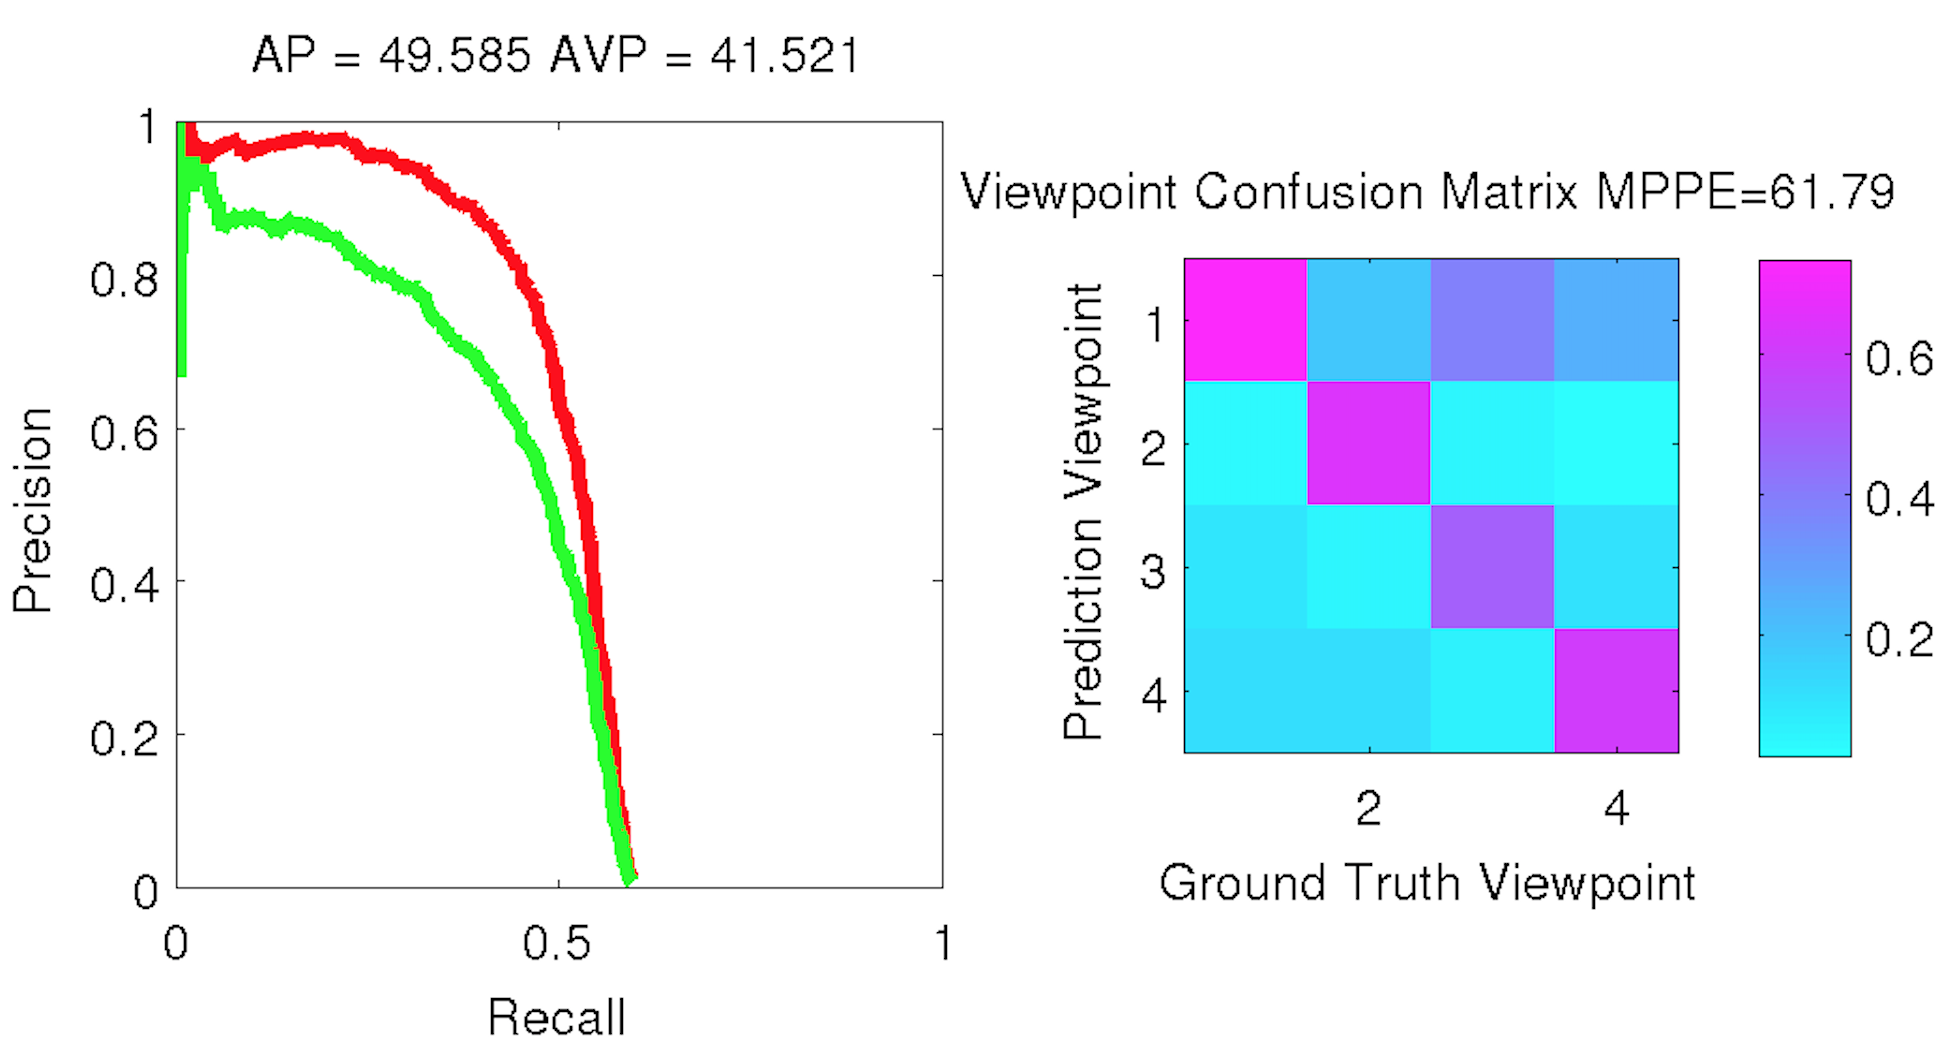
\includegraphics[width=0.49\linewidth]{car_cnn4_crop.png} &   
  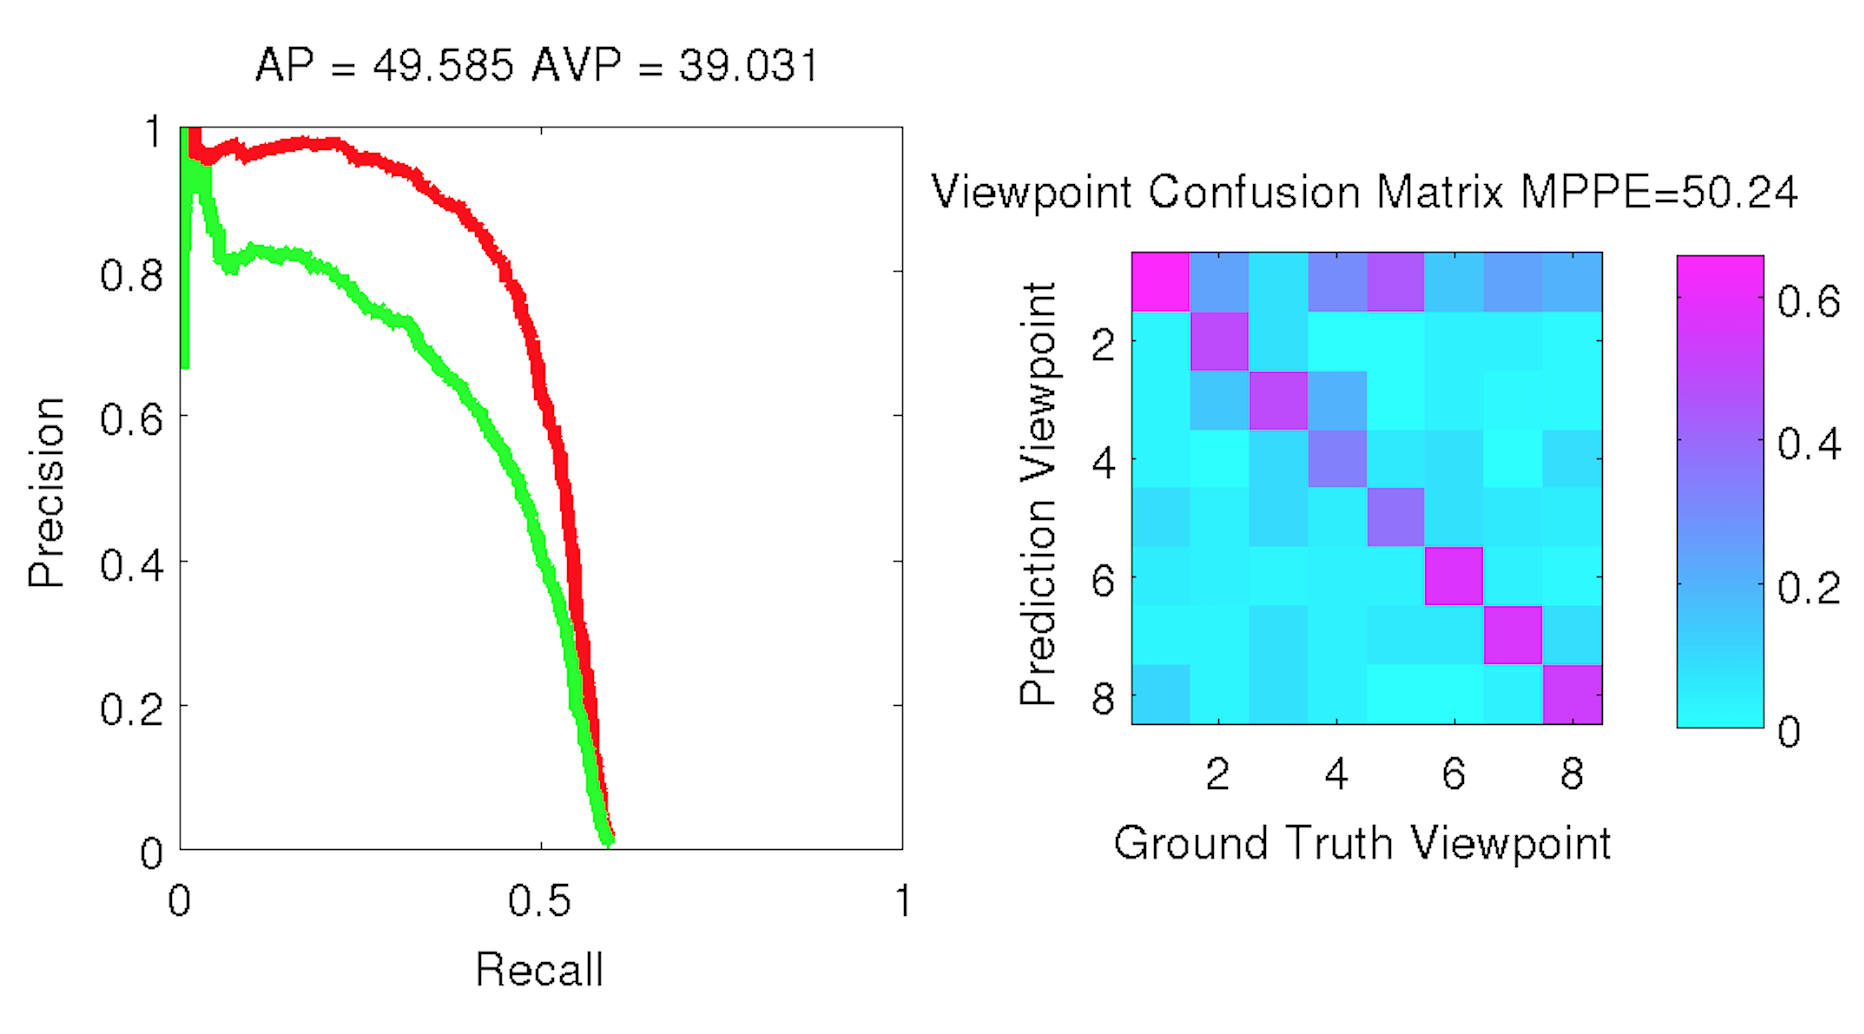
\includegraphics[width=0.49\linewidth]{car_cnn8_crop.png} \\   
  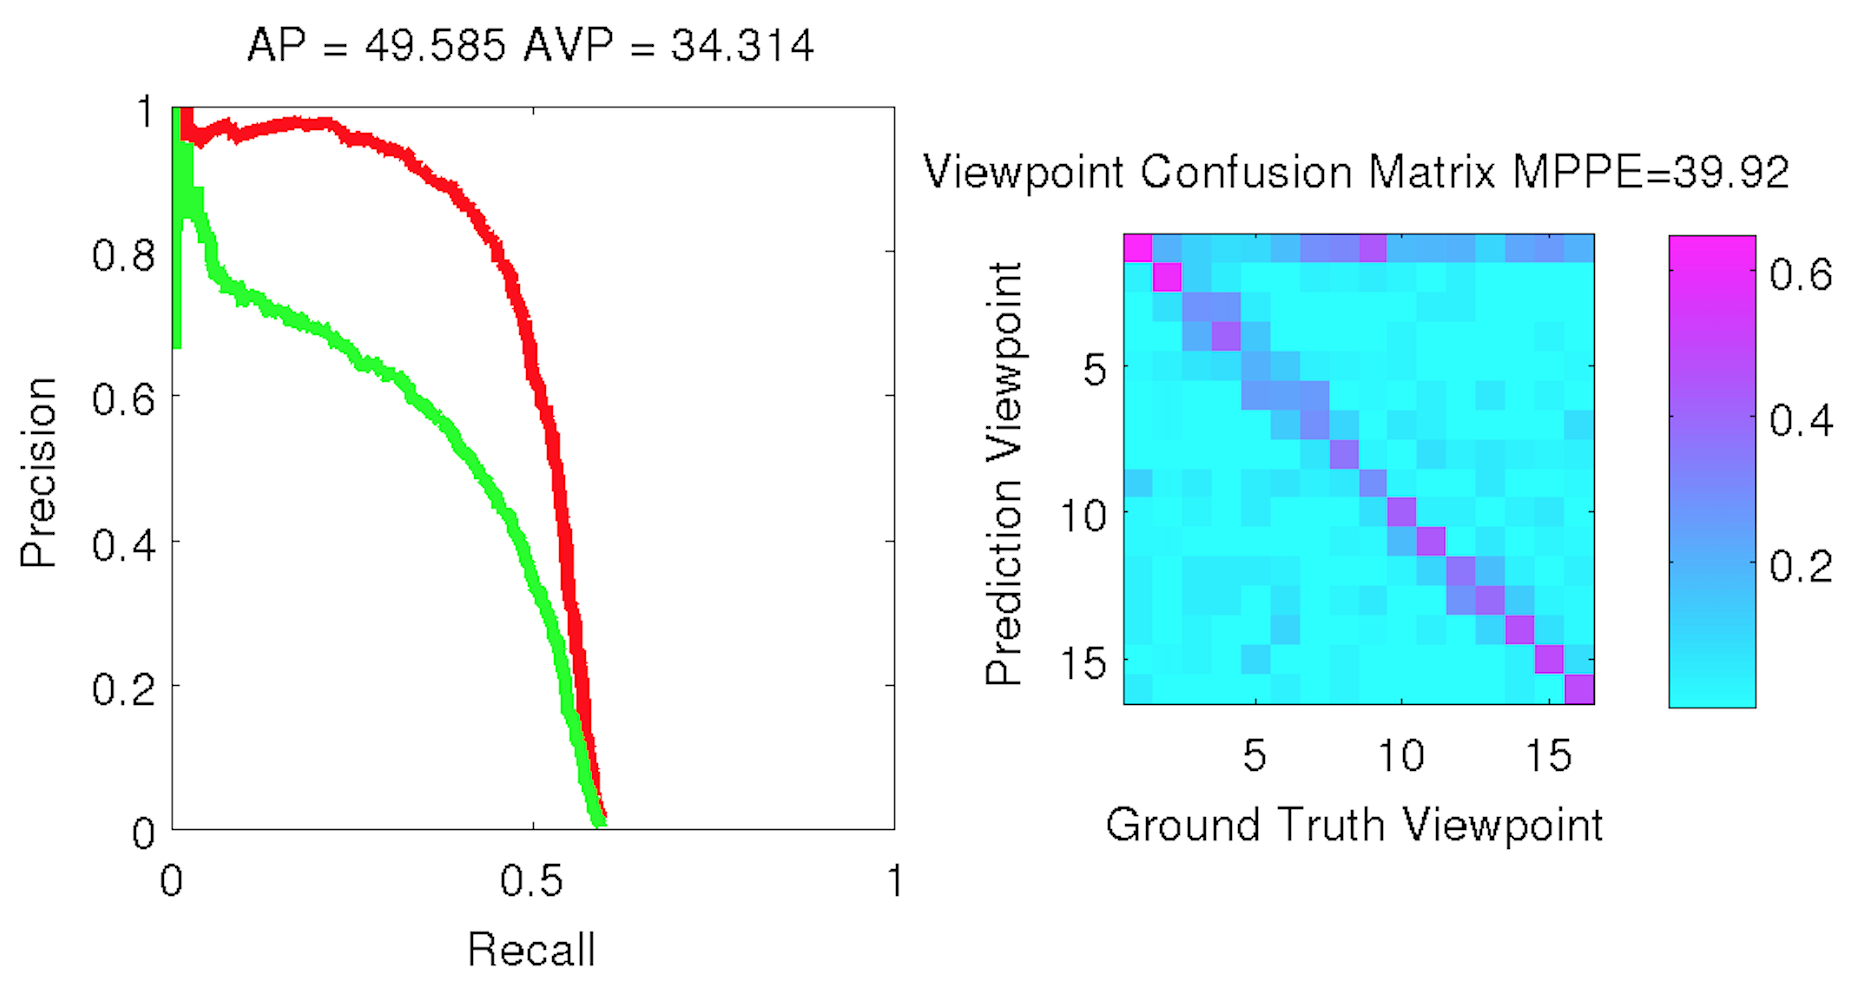
\includegraphics[width=0.49\linewidth]{car_cnn16_crop.png} &   
  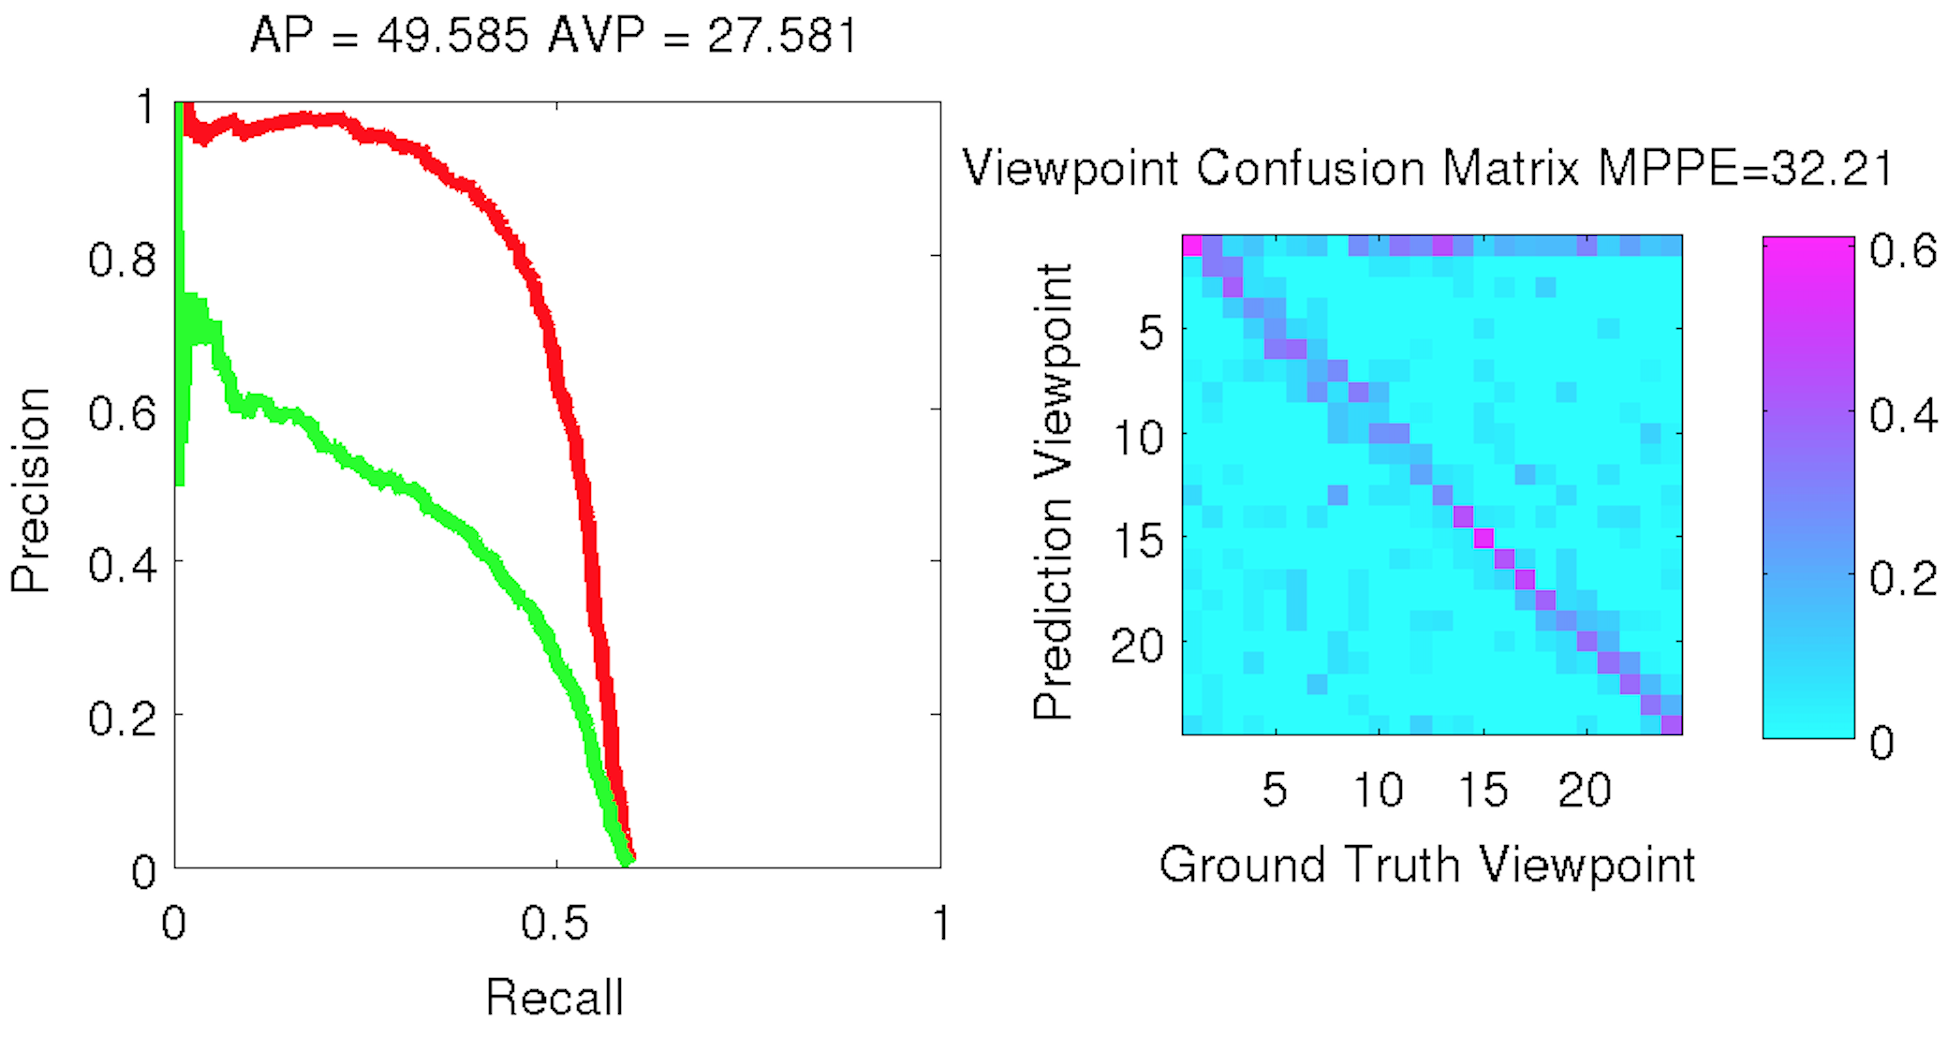
\includegraphics[width=0.49\linewidth]{car_cnn24_crop.png} \\   
%  \hline
\end{tabular}
\caption{Average Precision (AP)(red) and Average Viewpoint Precision (AVP)(green)
  and viewpoint confusion table on PASCAL 12 car validation set using
  R-CNN + Ours (full). From the top left, 4 views, 8 views, 16 views
  and 24 views.}
 % Since our method only augment the object detection,
 %  the AP remains the same for all cases. As we increase the viewpoint
 %  estimation, the AVP decreases. Note that since we estimate null
 %  viewpoint if our method fails to find match, there are more 0
 %  viewpoint predictions (top row of confusion matrices) }
  \label{fig:car_cnn_ap}
\end{figure}

\vspace{-0.1in}
\paragraph{Robustness.}
% Generic object detectors give overlapping detection bounding boxes of the same object which can be handled by non maximal suppression. For these overlapping detections, 
While the R-CNN detector~\cite{Girshick14} is highly robust to
variations in object appearance and even occlusion and truncation,
the resulting bounding box detections vary largely in the object
portions that they contain, which provides a major challenge to any
method that uses these detections as an input for further processing,
such as ours.
%
In order to accommodate this variability, we add a considerable context
region around the proposed bounding boxes before running our method.
We assume that the object can be arbitrarily truncated by the bounding
box and search all plausible scales and translations. This can be
efficiently computed using FFT-based convolution
(Section. \ref{sec:fft}).

Fig.~\ref{fig:stability} visualizes example outputs of our method when
starting from different proposed R-CNN bounding boxes. As can be seen
from the figure, although the input bounding boxes (cyan) are often
irregular and contain truncated objects, our method reliably
generates a reasonable prediction of pose, translation, scale and CAD
model (magenta bounding boxes enclose the output of our system).

\begin{figure}[h]
\setlength\tabcolsep{5pt}
\begin{tabular}{cc}
  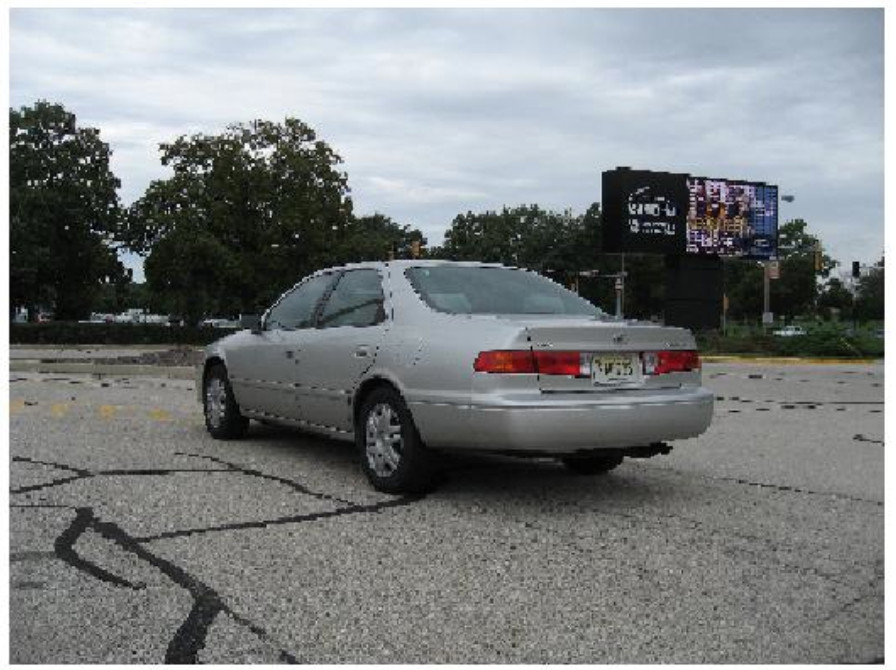
\includegraphics[width=0.45\linewidth]{car_pascal/1.png} &   
  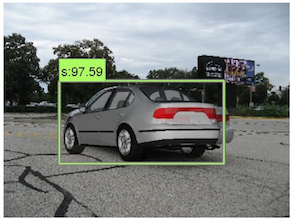
\includegraphics[width=0.45\linewidth]{car_pascal/2.png} \\   
  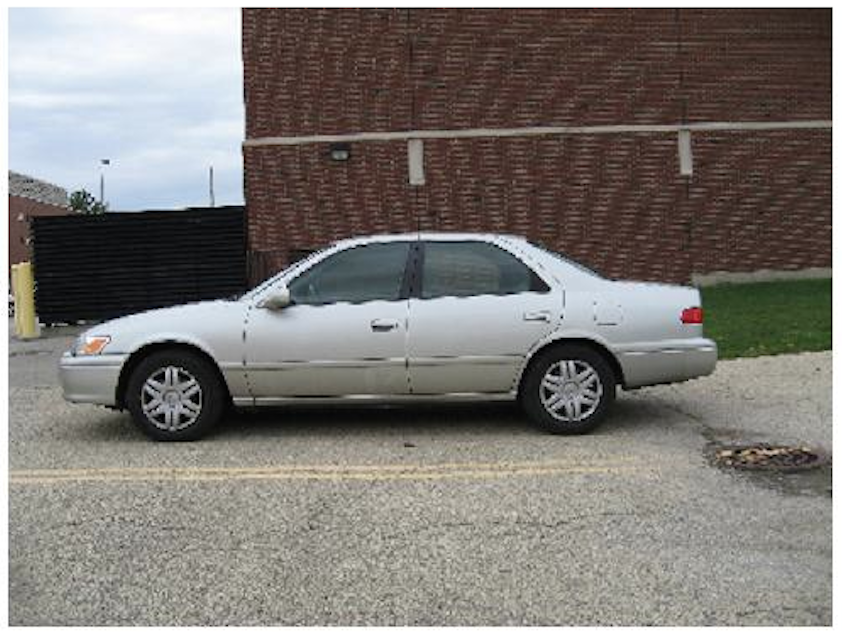
\includegraphics[width=0.45\linewidth]{car_pascal/3.png} &   
  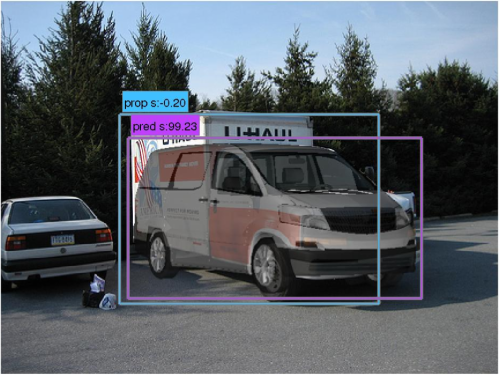
\includegraphics[width=0.45\linewidth]{car_pascal/4.png} \\   
\end{tabular}
\caption{Robustness of our method against irregular and truncated
  R-CNN detection proposals (cyan).}
  % \cite{Girshick14}. Blue box is the R-CNN detection that is feed into
  % the system as initial detection. Purple box and overlaid rendering
  % is the final output of the system. Note that for various overlapping
  % bounding boxes, our system accurately estimated the reasonable
  % result}
  \label{fig:stability}
\end{figure}


% For qualitative examples, we put hand-picked results from our method Fig. \ref{fig:car} and Fig. \ref{fig:bicycle}.

% \begin{figure*}[h]
% \setlength\tabcolsep{5pt}
% \begin{tabular}{|c|c|c|}
%     \hline
%   \includegraphics[width=0.325\textwidth]{car/PASCAL_car_val_init_0_Car_each_27_lim_250_lam_0_150_a_24_e_3_y_1_f_1_scale_2_00_sbin_6_level_15_skp_n_server_101_img_39.jpg} &   
%   \includegraphics[width=0.325\textwidth]{car/PASCAL_car_val_init_0_Car_each_27_lim_250_lam_0_150_a_24_e_3_y_1_f_1_scale_2_00_sbin_6_level_15_skp_n_server_101_img_78.jpg} & 
%   \includegraphics[width=0.325\textwidth]{car/PASCAL_car_val_init_0_Car_each_27_lim_250_lam_0_150_a_24_e_3_y_1_f_1_scale_2_00_sbin_6_level_15_skp_n_server_101_img_85.jpg} \\[-15pt]
% (a) & (b) & (c) \\[0pt]
% \hline
%   \includegraphics[width=0.325\textwidth]{car/PASCAL_car_val_init_0_Car_each_27_lim_250_lam_0_150_a_24_e_3_y_1_f_1_scale_2_00_sbin_6_level_15_skp_n_server_101_img_338.jpg} &   
%   \includegraphics[width=0.325\textwidth]{car/PASCAL_car_val_init_0_Car_each_27_lim_250_lam_0_150_a_24_e_3_y_1_f_1_scale_2_00_sbin_6_level_15_skp_n_server_101_img_360.jpg} & 
%   \includegraphics[width=0.325\textwidth]{car/PASCAL_car_val_init_0_Car_each_27_lim_250_lam_0_150_a_24_e_3_y_1_f_1_scale_2_00_sbin_6_level_15_skp_n_server_101_img_414.jpg} \\[-15pt]
% (d) & (e) & (f) \\[0pt]
% \hline
%   \includegraphics[width=0.325\textwidth]{car/PASCAL_car_val_init_0_Car_each_27_lim_250_lam_0_150_a_24_e_3_y_1_f_1_scale_2_00_sbin_6_level_15_skp_n_server_101_img_418.jpg} &   
%   \includegraphics[width=0.325\textwidth]{car/PASCAL_car_val_init_0_Car_each_27_lim_250_lam_0_150_a_24_e_3_y_1_f_1_scale_2_00_sbin_6_level_15_skp_n_server_101_img_1049.jpg} & 
%   \includegraphics[width=0.325\textwidth]{car/PASCAL_car_val_init_0_Car_each_27_lim_250_lam_0_150_a_24_e_3_y_1_f_1_scale_2_00_sbin_6_level_15_skp_n_server_101_img_1242.jpg} \\[-15pt]
% (g) & (h) & (i) \\[0pt]
% \hline
%   \includegraphics[width=0.325\textwidth]{car/PASCAL_car_val_init_0_Car_each_27_lim_250_lam_0_150_a_24_e_3_y_1_f_1_scale_2_00_sbin_6_level_15_skp_n_server_101_img_1244.jpg} &   
%   \includegraphics[width=0.325\textwidth]{car/PASCAL_car_val_init_0_Car_each_27_lim_250_lam_0_150_a_24_e_3_y_1_f_1_scale_2_00_sbin_6_level_15_skp_n_server_101_img_1261.jpg} & 
%   \includegraphics[width=0.325\textwidth]{car/PASCAL_car_val_init_0_Car_each_27_lim_250_lam_0_150_a_24_e_3_y_1_f_1_scale_2_00_sbin_6_level_15_skp_n_server_101_img_1452.jpg} \\[-15pt]
% (j) & (k) & (l) \\[0pt]
% \hline
%   \includegraphics[width=0.325\textwidth]{car/PASCAL_car_val_init_0_Car_each_27_lim_250_lam_0_150_a_24_e_3_y_1_f_1_scale_2_00_sbin_6_level_15_skp_n_server_101_img_1467.jpg} &   
%   \includegraphics[width=0.325\textwidth]{car/PASCAL_car_val_init_0_Car_each_27_lim_250_lam_0_150_a_24_e_3_y_1_f_1_scale_2_00_sbin_6_level_15_skp_n_server_101_img_1553.jpg} & 
%   \includegraphics[width=0.325\textwidth]{car/PASCAL_car_val_init_0_Car_each_27_lim_250_lam_0_150_a_24_e_3_y_1_f_1_scale_2_00_sbin_6_level_15_skp_n_server_101_img_1597.jpg} \\[-15pt]
% (m) & (n) & (o) \\[3pt]
% \hline
% \end{tabular}
%   \caption{Selected detections from PASCAL 07 Car categories. From the left, (1) original image, (2) overlaid true positive CAD models, (3) overlaid true positive CAD models with bounding boxes, (4) overlaid false positive CAD models with bounding boxes. Bounding box is colored from red (high confidence) to blue (low confidence) }
%   \label{fig:car}
% \end{figure*}
% \begin{figure*}[h]
% \setlength\tabcolsep{5pt}
% \begin{tabular}{|c|c|c|}
%     \hline
%   \includegraphics[width=0.325\textwidth]{bicycle/PASCAL_bicycle_val_init_0_Bicycle_each_4_lim_250_lam_0_150_a_48_e_4_y_5_f_1_scale_2_00_sbin_6_level_15_skp_n_server_102_img_459.jpg} &   
%   \includegraphics[width=0.325\textwidth]{bicycle/PASCAL_bicycle_val_init_0_Bicycle_each_4_lim_250_lam_0_150_a_48_e_4_y_5_f_1_scale_2_00_sbin_6_level_15_skp_n_server_102_img_1300.jpg} &   
%   \includegraphics[width=0.325\textwidth]{bicycle/PASCAL_bicycle_val_init_0_Bicycle_each_4_lim_250_lam_0_150_a_48_e_4_y_5_f_1_scale_2_00_sbin_6_level_15_skp_n_server_102_img_539.jpg} \\[-15pt]
% (a) & (b) & (c) \\[0pt]
% \hline
%   \includegraphics[width=0.325\textwidth]{bicycle/PASCAL_bicycle_val_init_0_Bicycle_each_4_lim_250_lam_0_150_a_48_e_4_y_5_f_1_scale_2_00_sbin_6_level_15_skp_n_server_102_img_35.jpg} &   
%   \includegraphics[width=0.325\textwidth]{bicycle/PASCAL_bicycle_val_init_0_Bicycle_each_4_lim_250_lam_0_150_a_48_e_4_y_5_f_1_scale_2_00_sbin_6_level_15_skp_n_server_102_img_83.jpg} &   
%   \includegraphics[width=0.325\textwidth]{bicycle/PASCAL_bicycle_val_init_0_Bicycle_each_4_lim_250_lam_0_150_a_48_e_4_y_5_f_1_scale_2_00_sbin_6_level_15_skp_n_server_102_img_131.jpg} \\[-15pt]
% (d) & (e) & (f) \\[0pt]
% \hline
%   \includegraphics[width=0.325\textwidth]{bicycle/PASCAL_bicycle_val_init_0_Bicycle_each_4_lim_250_lam_0_150_a_48_e_4_y_5_f_1_scale_2_00_sbin_6_level_15_skp_n_server_102_img_175.jpg} &   
%   \includegraphics[width=0.325\textwidth]{bicycle/PASCAL_bicycle_val_init_0_Bicycle_each_4_lim_250_lam_0_150_a_48_e_4_y_5_f_1_scale_2_00_sbin_6_level_15_skp_n_server_102_img_210.jpg} &   
%   \includegraphics[width=0.325\textwidth]{bicycle/PASCAL_bicycle_val_init_0_Bicycle_each_4_lim_250_lam_0_150_a_48_e_4_y_5_f_1_scale_2_00_sbin_6_level_15_skp_n_server_102_img_233.jpg} \\[-15pt]
% (g) & (h) & (i) \\[0pt]
% \hline
%   \includegraphics[width=0.325\textwidth]{bicycle/PASCAL_bicycle_val_init_0_Bicycle_each_4_lim_250_lam_0_150_a_48_e_4_y_5_f_1_scale_2_00_sbin_6_level_15_skp_n_server_102_img_322.jpg} &   
%   \includegraphics[width=0.325\textwidth]{bicycle/PASCAL_bicycle_val_init_0_Bicycle_each_4_lim_250_lam_0_150_a_48_e_4_y_5_f_1_scale_2_00_sbin_6_level_15_skp_n_server_102_img_348.jpg} &   
%   \includegraphics[width=0.325\textwidth]{bicycle/PASCAL_bicycle_val_init_0_Bicycle_each_4_lim_250_lam_0_150_a_48_e_4_y_5_f_1_scale_2_00_sbin_6_level_15_skp_n_server_102_img_375.jpg} \\[-15pt]
% (j) & (k) & (l) \\[0pt]
% \hline
%   \includegraphics[width=0.325\textwidth]{bicycle/PASCAL_bicycle_val_init_0_Bicycle_each_4_lim_250_lam_0_150_a_48_e_4_y_5_f_1_scale_2_00_sbin_6_level_15_skp_n_server_102_img_400.jpg} &   
%   \includegraphics[width=0.325\textwidth]{bicycle/PASCAL_bicycle_val_init_0_Bicycle_each_4_lim_250_lam_0_150_a_48_e_4_y_5_f_1_scale_2_00_sbin_6_level_15_skp_n_server_102_img_434.jpg} &   
%   \includegraphics[width=0.325\textwidth]{bicycle/PASCAL_bicycle_val_init_0_Bicycle_each_4_lim_250_lam_0_150_a_48_e_4_y_5_f_1_scale_2_00_sbin_6_level_15_skp_n_server_102_img_459.jpg} \\[-15pt]
% (m) & (n) & (o) \\[3pt]
% \hline
% \end{tabular}
%   \caption{Selected detections from PASCAL 12 Bike categories. From the left, (1) original image, (2) overlaid true positive CAD models, (3) overlaid true positive CAD models with bounding boxes, (4) overlaid false positive CAD models with bounding boxes. Bounding box is colored from red (high confidence) to blue (low confidence) }
%   \label{fig:bicycle}
% \end{figure*}


% \section{Object Detection with various Training Data}
% \section{Image Query}
